%!TEX root = ./main.tex
% ==============================================================================
% MASTER DOCUMENT PROPOSAL SKRIPSI
% Fakultas Sains dan Teknologi - Universitas Bahaudin Mudhary Madura
% Sesuai Buku Pedoman Penulisan Skripsi FST UNIBA Madura Revisi 2026
% ==============================================================================

\documentclass[12pt, a4paper, oneside]{report}

% 1. Pemuatan Modul Konfigurasi
% ==============================================================================
% PAKET-PAKET LATEX (PACKAGES)
% Proposal Skripsi Informatika FST UNIBA Madura
% ==============================================================================

% Pengaturan Margin & Ukuran Kertas Sesuai Pedoman FST UNIBA Madura 2026
\usepackage[
    a4paper,
    left=4cm,
    top=3cm,
    right=3cm,
    bottom=3cm,
    footskip=1.5cm,
    headheight=15pt
]{geometry}

% Tipografi: Times New Roman 12pt & Justifikasi Teks Rapi
\usepackage{mathptmx}
\usepackage[utf8]{inputenc}
\usepackage[T1]{fontenc}
\usepackage{microtype}

% Spasi dan Indentasi
\usepackage{setspace}
\usepackage{indentfirst} % Paragraf pertama setelah heading tetap menjorok masuk
\usepackage{enumitem}    % Pengendalian presisi spasi daftar (list/enumerate/itemize) tanpa space after/before

% Simbol & Rumus Matematika
\usepackage{amsmath}
\usepackage{amssymb}
\usepackage{amsfonts}

% Gambar dan Grafik
\usepackage{graphicx}
\usepackage{float}
\usepackage{tikz}
\usetikzlibrary{shapes.geometric, arrows.meta, positioning, fit, calc}

% Tabel Akademik
\usepackage{booktabs}
\usepackage{tabularx}
\usepackage{longtable}
\usepackage{multirow}
\usepackage{array}
\usepackage{colortbl}

% Format Judul Bab & Subbab
\usepackage{titlesec}
\usepackage{etoolbox}

% Header dan Footer (Penomoran Halaman)
\usepackage{fancyhdr}

% Keterangan Gambar & Tabel
\usepackage{caption}
\usepackage{subcaption}

% Penyorotan Kode Program (Syntax Highlighting)
\usepackage{listings}
\usepackage{xcolor}

% Pengaturan Daftar Isi, Gambar, dan Tabel
\usepackage{titletoc}

% Sitasi & Daftar Pustaka Gaya APA (American Psychological Association)
\usepackage[natbibapa]{apacite}

% Hyperlink dokumen PDF
\usepackage{hyperref}
\usepackage{url}

% ==============================================================================
% METADATA PROPOSAL SKRIPSI
% Fakultas Sains dan Teknologi - Universitas Bahaudin Mudhary Madura
% ==============================================================================

% Judul Skripsi (Bahasa Indonesia & Bahasa Inggris)
% Istilah bahasa asing dimiringkan (\textit{...}) agar taat kaidah bahasa baku
\newcommand{\skripsiJudul}{EVALUASI GENERALISASI DAN ADAPTASI LINTAS DOMAIN MODEL ANALISIS SENTIMEN BAHASA MADURA DARI DATASET NUSAX KE KOMENTAR TIKTOK}
\newcommand{\skripsiJudulEn}{CROSS-DOMAIN GENERALIZATION AND ADAPTATION EVALUATION OF MADURESE SENTIMENT ANALYSIS MODEL FROM NUSAX DATASET TO TIKTOK COMMENTS}

% Tipe Dokumen & Bidang Minat
\newcommand{\skripsiTipeDokumen}{PROPOSAL SKRIPSI}
\newcommand{\skripsiBidangMinat}{Sains Data dan Kecerdasan Artifisial}
\newcommand{\skripsiTujuanDokumen}{Diajukan untuk memenuhi persyaratan\\ Memperoleh gelar Sarjana Komputer}

% Identitas Penulis
\newcommand{\skripsiPenulis}{Muhammad Syawqi Muhtadabillah}
\newcommand{\skripsiNIM}{2302310276}

% Informasi Program Studi & Fakultas
\newcommand{\skripsiGelar}{Sarjana Komputer}
\newcommand{\skripsiSingkatanGelar}{S.Kom.}
\newcommand{\skripsiProdi}{Informatika}
\newcommand{\skripsiFakultas}{Fakultas Sains dan Teknologi}
\newcommand{\skripsiUniversitas}{Universitas K.H. Bahaudin Mudhary Madura}
\newcommand{\skripsiKota}{Sumenep}
\newcommand{\skripsiTahun}{2026}
\newcommand{\skripsiBulanTahun}{Mei 2026}

% Dosen Pembimbing
\newcommand{\skripsiPembimbingSatu}{Prof. Dr. Ir. Rachmad Hidayat, M.T., IPU., ASEAN Eng.}
\newcommand{\skripsiNIKPembimbingSatu}{19740619.201808.1.010}
\newcommand{\skripsiPembimbingDua}{Pyepit Rinekso Andriyanto, S.Kom., M.Kom.}
\newcommand{\skripsiNIKPembimbingDua}{19910225.202402.1.173}

% Pimpinan Fakultas & Program Studi
\newcommand{\skripsiDekan}{Emon Rifa'i, S.T., M.T.}
\newcommand{\skripsiKaprodi}{Zeinor Rahman, S.Pd., M.Pd.}
\newcommand{\skripsiNIKKaprodi}{19960306.202108.1.061}

% Tanggal Pengesahan (Format Bahasa Indonesia)
\newcommand{\tanggalIndonesia}{%
  \the\day\ \ifcase\month\or Januari\or Februari\or Maret\or April\or Mei\or Juni\or Juli\or Agustus\or September\or Oktober\or November\or Desember\fi\ \the\year%
}
\newcommand{\skripsiTanggalPengesahan}{\tanggalIndonesia}

% ==============================================================================
% PENGATURAN FORMATTING & TATA LETAK SKRIPSI
% Sesuai Pedoman Penulisan Skripsi FST UNIBA Madura 2026
% ==============================================================================

% 1. SPASI & INDENTASI
\onehalfspacing                      % Spasi antar baris 1.5
\setlength{\parindent}{0.75cm}       % Indent alinea baru 0.75 cm (7 ketukan)
\setlength{\parskip}{0pt}            % Jarak antar paragraf 0pt (tanpa spasi kosong ekstra)
\raggedbottom                        % Cegah peregangan vertikal LaTeX

% Pengaturan Spasi Daftar (List: Enumerate & Itemize) tanpa spasi ekstra
\setlist{
  nosep,                             % Hapus space before/after dan space ekstra antar butir
  topsep=0pt,
  partopsep=0pt,
  parsep=0pt,
  itemsep=0pt,
  leftmargin=0.75cm,                 % Indentasi sejajar alinea baru
  labelsep=0.25cm
}
\setlist[enumerate]{label=\arabic*., ref=\arabic*}
\setlist[itemize]{label=\textbullet}

% 2. PENAMAAN STRUKTUR DOKUMEN (BAHASA INDONESIA)
\renewcommand{\contentsname}{DAFTAR ISI}
\renewcommand{\listfigurename}{DAFTAR GAMBAR}
\renewcommand{\listtablename}{DAFTAR TABEL}
\renewcommand{\bibname}{DAFTAR PUSTAKA}
\renewcommand{\chaptername}{BAB}
\renewcommand{\appendixname}{LAMPIRAN}
\renewcommand{\figurename}{Gambar}
\renewcommand{\tablename}{Tabel}

% 3. FORMAT PENOMORAN PERSAMAAN, TABEL, DAN GAMBAR PER BAB
\renewcommand{\thechapter}{\Roman{chapter}}
\renewcommand{\thesection}{\arabic{chapter}.\arabic{section}}
\renewcommand{\thesubsection}{\arabic{chapter}.\arabic{section}.\arabic{subsection}}
\renewcommand{\theequation}{\arabic{chapter}-\arabic{equation}}
\renewcommand{\thefigure}{\arabic{chapter}.\arabic{figure}}
\renewcommand{\thetable}{\arabic{chapter}.\arabic{table}}

% 4. FORMAT JUDUL BAB, SUB-BAB, DAN SUB-SUB-BAB (TITLESEC)
\titleformat{\chapter}[display]
  {\singlespacing\centering\bfseries}
  {\fontsize{14pt}{18pt}\selectfont\MakeUppercase{\chaptername\ \thechapter}}
  {0.5em}
  {\fontsize{12pt}{16pt}\selectfont\MakeUppercase}

\titlespacing*{\chapter}{0pt}{-35pt}{1.5em}

% Format Sub-bab (Section)
\titleformat{\section}
  {\singlespacing\bfseries\fontsize{12pt}{16pt}\selectfont}
  {\thesection}
  {0.75em}
  {}
\titlespacing*{\section}{0pt}{1.0em}{0.2em}

% Format Sub-sub-bab (Subsection)
\titleformat{\subsection}
  {\singlespacing\bfseries\fontsize{12pt}{16pt}\selectfont}
  {\thesubsection}
  {0.75em}
  {}
\titlespacing*{\subsection}{0pt}{0.8em}{0.2em}

% Eliminasi jeda spasi ekstra jika \subsection langsung mengikuti \section
\newif\ifdirectlyaftersection
\directlyaftersectionfalse

\pretocmd{\section}{\directlyaftersectiontrue}{}{}
\pretocmd{\subsection}{%
  \ifdirectlyaftersection
    \vspace{-0.85em}%
    \directlyaftersectionfalse
  \fi
}{}{}

\makeatletter
\everypar=\expandafter{\the\everypar \directlyaftersectionfalse}
\makeatother

% 5. LOGIKA PENOMORAN HALAMAN (FANCYHDR)
\fancypagestyle{frontstyle}{
  \fancyhf{}
  \renewcommand{\headrulewidth}{0pt}
  \renewcommand{\footrulewidth}{0pt}
  \fancyfoot[C]{\thepage}
}

\fancypagestyle{mainstyle}{
  \fancyhf{}
  \renewcommand{\headrulewidth}{0pt}
  \renewcommand{\footrulewidth}{0pt}
  \fancyhead[R]{\thepage}
}

\fancypagestyle{plain}{
  \fancyhf{}
  \renewcommand{\headrulewidth}{0pt}
  \renewcommand{\footrulewidth}{0pt}
  \fancyfoot[C]{\thepage}
}

% 6. PENGATURAN SPASI & CAPTION OBJEK GAMBAR & TABEL
\setlength{\floatsep}{4pt plus 1pt minus 1pt}
\setlength{\textfloatsep}{6pt plus 1pt minus 1pt}
\setlength{\intextsep}{0pt}
\setlength{\dblfloatsep}{4pt plus 1pt minus 1pt}
\setlength{\dbltextfloatsep}{6pt plus 1pt minus 1pt}

\captionsetup[table]{
  labelfont={bf},
  textfont={normalfont},
  justification=centering,
  labelsep=space,
  position=bottom,
  aboveskip=4pt,
  belowskip=2pt
}

\captionsetup[figure]{
  labelfont={bf},
  textfont={normalfont},
  justification=centering,
  labelsep=space,
  position=bottom,
  aboveskip=4pt,
  belowskip=0pt
}

% 7. FORMAT KUTIPAN DAFTAR PUSTAKA APA
\AtBeginDocument{
  \renewcommand{\bibname}{DAFTAR PUSTAKA}
  \renewcommand{\refname}{DAFTAR PUSTAKA}
}
\setlength{\bibhang}{0.75cm}
\setlength{\bibsep}{6.9pt}

% 8. PENYOROTAN KODE PROGRAM (LISTINGS)
\definecolor{codegray}{rgb}{0.5,0.5,0.5}
\definecolor{backcolour}{rgb}{0.97,0.97,0.97}
\definecolor{primaryblue}{rgb}{0.0,0.2,0.6}
\definecolor{stringgreen}{rgb}{0.1,0.5,0.2}

\lstdefinestyle{skripsicode}{
  backgroundcolor=\color{backcolour},
  commentstyle=\color{codegray}\itshape,
  keywordstyle=\color{primaryblue}\bfseries,
  numberstyle=\tiny\color{codegray},
  stringstyle=\color{stringgreen},
  basicstyle=\ttfamily\footnotesize\singlespacing,
  breakatwhitespace=false,
  breaklines=true,
  captionpos=b,
  keepspaces=true,
  numbers=left,
  numbersep=7pt,
  showspaces=false,
  showstringspaces=false,
  showtabs=false,
  tabsize=2,
  frame=single,
  rulecolor=\color{lightgray}
}
\lstset{style=skripsicode}

% 9. HYPERLINK SETUP
\hypersetup{
  colorlinks=true,
  linkcolor=black,
  citecolor=black,
  urlcolor=blue,
  pdfborder={0 0 0}
}

% 10. FORMAT DAFTAR ISI, DAFTAR GAMBAR, DAN DAFTAR TABEL (TITLETOC)
\contentsmargin[1.5em]{1.2em}

\titlecontents{chapter}[0pt]
  {\vspace{0.35em}\bfseries}
  {BAB \thecontentslabel\ }
  {}
  {\titlerule*[0.28pc]{.}\contentspage}

\titlecontents{section}[1.6cm]
  {\normalfont}
  {\contentslabel[\thecontentslabel]{0.8cm}}
  {}
  {\titlerule*[0.28pc]{.}\contentspage}

\titlecontents{subsection}[2.8cm]
  {\normalfont}
  {\contentslabel[\thecontentslabel]{1.2cm}}
  {}
  {\titlerule*[0.28pc]{.}\contentspage}

\titlecontents{figure}[2.5cm]
  {\normalfont}
  {\contentslabel[\textbf{Gambar \thecontentslabel}]{2.5cm}}
  {}
  {\titlerule*[0.28pc]{.}\contentspage}

\titlecontents{table}[2.2cm]
  {\normalfont}
  {\contentslabel[\textbf{Tabel \thecontentslabel}]{2.2cm}}
  {}
  {\titlerule*[0.28pc]{.}\contentspage}


\begin{document}

% ==============================================================================
% BAGIAN AWAL (FRONTMATTER)
% ==============================================================================
\pagestyle{empty}
\hypersetup{pageanchor=false}

% Halaman Sampul (Cover Proposal)
% ==============================================================================
% HALAMAN SAMPUL (COVER)
% Sesuai Lampiran 1b Pedoman Penulisan Skripsi FST UNIBA Madura 2026
% ==============================================================================

\begin{titlepage}
\begin{center}
    \singlespacing
    
    % Judul Skripsi (Kapital, Tebal, 12pt proporsional)
    {\fontsize{12pt}{16pt}\selectfont \bfseries \skripsiJudul}
    
    \vspace{1.5cm}
    
    % Tulisan Tipe Dokumen (PROPOSAL SKRIPSI) & Bidang Minat
    {\fontsize{12pt}{16pt}\selectfont \bfseries \MakeUppercase{\skripsiTipeDokumen}}\\[0.25cm]
    {\fontsize{12pt}{16pt}\selectfont \skripsiBidangMinat}
    
    \vspace{0.9cm}
    
    % Kalimat Persyaratan (12pt reguler)
    {\fontsize{12pt}{16pt}\selectfont
    \skripsiTujuanDokumen
    }
    
    \vspace{1.2cm}
    
    % Logo Universitas Bahaudin Mudhary Madura
    
\includegraphics[width=4.0cm]{figures/logo-uniba.png}
    
    \vspace{1.2cm}
    
    % Identitas Mahasiswa (Nama tebal, NIM reguler)
    {\fontsize{12pt}{16pt}\selectfont \bfseries \MakeUppercase{\skripsiPenulis}}\\
    \vspace{0.2cm}
    {\fontsize{12pt}{16pt}\selectfont NIM. \skripsiNIM}
    
    \vfill
    
    % Identitas Institusi
    {\fontsize{12pt}{16pt}\selectfont \bfseries
    PROGRAM STUDI \MakeUppercase{\skripsiProdi}\\
    \MakeUppercase{\skripsiFakultas}\\
    \MakeUppercase{\skripsiUniversitas}\\
    \MakeUppercase{\skripsiKota}\\
    \skripsiTahun
    }

\end{center}
\end{titlepage}


% Aktifkan pageanchor untuk hyperlink dokumen PDF
\hypersetup{pageanchor=true}

% Lembar Pengesahan Dosen Pembimbing (Halaman ii)
% ==============================================================================
% LEMBAR PENGESAHAN DOSEN PEMBIMBING
% Sesuai Format Pedoman Skripsi FST UNIBA Madura 2026
% ==============================================================================

\clearpage
\phantomsection
\pagenumbering{roman}
\setcounter{page}{2}
\pagestyle{frontstyle}
\addcontentsline{toc}{chapter}{LEMBAR PENGESAHAN}

\begin{center}
    \singlespacing
    
    {\fontsize{12pt}{16pt}\selectfont \bfseries LEMBAR PENGESAHAN}
    
    \vspace{0.65cm}
    
    {\fontsize{12pt}{16pt}\selectfont \bfseries \skripsiJudul}
    
    \vspace{0.6cm}
    
    {\fontsize{12pt}{16pt}\selectfont \bfseries \MakeUppercase{\skripsiTipeDokumen}}\\[0.15cm]
    {\fontsize{12pt}{16pt}\selectfont \skripsiBidangMinat}
    
    \vspace{0.55cm}
    
    {\fontsize{12pt}{16pt}\selectfont
    \skripsiTujuanDokumen
    }
    
    \vspace{0.6cm}
    
    % Logo Universitas Bahaudin Mudhary Madura
    
\includegraphics[width=3.5cm]{figures/logo-uniba.png}
    
    \vspace{0.6cm}
    
    {\fontsize{12pt}{16pt}\selectfont \MakeUppercase{\skripsiPenulis}}\\[0.12cm]
    {\fontsize{12pt}{16pt}\selectfont NIM. \skripsiNIM}
    
    \vspace{0.6cm}
    
    {\fontsize{12pt}{16pt}\selectfont
    Proposal Skripsi ini telah disetujui oleh dosen pembimbing\\
    pada tanggal \dots\ \dots\ \skripsiTahun
    }
    
    \vspace{0.95cm}
    
    % Kolom Pembimbing I dan II
    \noindent
    \begin{minipage}[t]{0.48\textwidth}
        \centering
        Dosen Pembimbing I\\[1.6cm]
        \underline{Prof. Dr. Ir. Rachmad Hidayat, M.T.,}\\
        \underline{IPU., ASEAN Eng.}\\[2pt]
        NIP. \skripsiNIKPembimbingSatu
    \end{minipage}\hfill
    \begin{minipage}[t]{0.48\textwidth}
        \centering
        Dosen Pembimbing II\\[1.6cm]
        \underline{Pyepit Rinekso Andriyanto,}\\
        \underline{S.Kom., M.Kom.}\\[2pt]
        NIP. \skripsiNIKPembimbingDua
    \end{minipage}
    
    \vspace{0.95cm}
    
    % Mengetahui Kaprodi
    Mengetahui,\\
    Ketua Program Studi\\[1.6cm]
    \underline{\skripsiKaprodi}\\[2pt]
    NIP. \skripsiNIKKaprodi

\end{center}


% Kata Pengantar (Halaman iii)
% ==============================================================================
% KATA PENGANTAR
% Sesuai Format Pedoman Skripsi FST UNIBA Madura 2026
% ==============================================================================

\clearpage
\phantomsection
\pagestyle{frontstyle}
\addcontentsline{toc}{chapter}{KATA PENGANTAR}

\begin{center}
    {\fontsize{14pt}{18pt}\selectfont \bfseries KATA PENGANTAR}
\end{center}

\vspace{0.3cm}

\textit{Alhamdulillahi Rabbil ’Alamin}, segala puja dan puji syukur penulis panjatkan kehadirat Allah SWT atas berkah, rahmat, dan taufik-Nya, sehingga penulis dapat menyelesaikan penyusunan proposal skripsi yang berjudul \textbf{“\skripsiJudul”} ini dengan baik. Naskah proposal ini disusun sebagai salah satu syarat untuk memenuhi ketentuan dalam kurikulum serta menyelesaikan jenjang studi guna memperoleh gelar \skripsiGelar\ (\skripsiSingkatanGelar) pada Program Studi \skripsiProdi, \skripsiFakultas, \skripsiUniversitas.

Keberhasilan dalam merumuskan dan menyelesaikan proposal skripsi ini tentunya tidak terlepas dari bimbingan, petunjuk, arahan, saran, serta dukungan moral yang sangat berharga dari berbagai pihak. Oleh karena itu, melalui lembar ini, penulis menyampaikan rasa hormat dan terima kasih yang setulus-tulusnya kepada:

\begin{enumerate}\singlespacing\setlength{\itemsep}{1.5pt}\setlength{\parsep}{0pt}\setlength{\topsep}{2pt}
    \item Bapak \skripsiDekan, selaku Dekan Fakultas Sains dan Teknologi Universitas K.H. Bahaudin Mudhary Madura.
    \item Bapak Mohammad Iqbal Bachtiar, S.T., M.T., selaku Wakil Dekan Fakultas Sains dan Teknologi Universitas K.H. Bahaudin Mudhary Madura.
    \item Bapak \skripsiKaprodi, selaku Ketua Program Studi \skripsiProdi\ Universitas K.H. Bahaudin Mudhary Madura atas bimbingan dan dorongan akademis yang senantiasa diberikan.
    \item Bapak \skripsiPembimbingSatu, selaku Dosen Pembimbing I yang telah meluangkan banyak waktu, tenaga, pemikiran, serta arahan ilmiah yang kritis dan konstruktif dalam penyempurnaan gagasan penelitian ini.
    \item Bapak \skripsiPembimbingDua, selaku Dosen Pembimbing II atas ketelitian, bimbingan teknis perancangan metodologi, saran metodis, dan motivasi yang senantiasa diberikan kepada penulis.
    \item Seluruh Bapak dan Ibu Dosen serta Tenaga Kependidikan Program Studi \skripsiProdi\ Fakultas Sains dan Teknologi Universitas K.H. Bahaudin Mudhary Madura atas transfer ilmu pengetahuan dan fasilitas akademik selama perkuliahan.
    \item Teristimewa kepada Kedua Orang Tua tercinta, Ayahanda dan Ibunda, serta segenap keluarga besar atas doa yang tiada henti, cinta kasih, keikhlasan, dan pengorbanan tanpa batas yang menjadi sumber kekuatan utama bagi penulis.
    \item Rekan-rekan mahasiswa seperjuangan Program Studi \skripsiProdi\ angkatan 2023 atas diskusi, kebersamaan, dan dukungan semangat selama proses perkuliahan dan riset.
    \item Seluruh pihak yang telah memberikan kontribusi, baik secara langsung maupun tidak langsung, yang tidak dapat penulis sebutkan satu per satu.
\end{enumerate}

Penulis menyadari bahwa naskah proposal skripsi ini masih memiliki keterbatasan dan ketidaksempurnaan. Oleh sebab itu, penulis senantiasa terbuka menerima kritik objektif, evaluasi ilmiah, serta saran konstruktif dari dosen penguji dan pembaca demi penyempurnaan naskah dan pelaksanaan eksperimen penelitian ke depan. Semoga karya ini mampu memberikan kontribusi nyata bagi pengembangan ilmu pengetahuan di bidang pemrosesan bahasa alami daerah berdaya komputasi rendah (\textit{low-resource language processing}) serta bermanfaat bagi masyarakat.

\vspace{0.3cm}

\begin{flushright}
\begin{tabular}{l}
    \skripsiKota, \dots\ \dots\ \skripsiTahun\\[1.4cm]
    \skripsiPenulis
\end{tabular}
\end{flushright}


% Daftar Isi
\clearpage
\phantomsection
\addcontentsline{toc}{chapter}{DAFTAR ISI}
{\singlespacing
\tableofcontents}

% Daftar Tabel (Sesuai Pedoman FST 2026: Daftar Tabel mendahului Daftar Gambar)
\clearpage
\phantomsection
\addcontentsline{toc}{chapter}{DAFTAR TABEL}
{\singlespacing
\listoftables}

% Daftar Gambar
\clearpage
\phantomsection
\addcontentsline{toc}{chapter}{DAFTAR GAMBAR}
{\singlespacing
\listoffigures}

% Daftar Simbol (Sesuai Pedoman FST 2026: Lampiran 12)
\clearpage
\phantomsection
\addcontentsline{toc}{chapter}{DAFTAR SIMBOL}
% ==============================================================================
% DAFTAR SIMBOL DAN LAMBANG
% Sesuai Pedoman Penulisan Skripsi FST UNIBA Madura 2026 (Lampiran 12)
% ==============================================================================

\clearpage
\phantomsection
\pagestyle{frontstyle}

\begin{center}
    {\fontsize{14pt}{18pt}\selectfont \bfseries DAFTAR SIMBOL}
\end{center}

\vspace{0.5cm}

\noindent\begin{longtable}{|>{\centering\arraybackslash}p{2.4cm}|>{\raggedright\arraybackslash}p{8.0cm}|>{\centering\arraybackslash}p{2.6cm}|}
    \hline
    \rowcolor[gray]{0.85}
    \textbf{Simbol} & \textbf{Keterangan / Besaran} & \textbf{Satuan / Dimensi} \\
    \hline
    \endfirsthead
    \hline
    \rowcolor[gray]{0.85}
    \textbf{Simbol} & \textbf{Keterangan / Besaran} & \textbf{Satuan / Dimensi} \\
    \hline
    \endhead
    \hline
    \endfoot

    % Simbol Matematika & Pemodelan Transformer
    $\text{Attention}(\cdot)$ & Fungsi pemetaan atensi terbobot (\textit{Scaled Dot-Product Attention}) & Skalar / Matriks \\
    \hline
    $\mathbf{b}$ & Vektor bias pada lapisan klasifikasi linier & $\mathbb{R}^{3}$ \\
    \hline
    $C$ & Jumlah total kelas kategori sentimen target ($C = 3$) & Bilangan Bulat \\
    \hline
    $c$ & Indeks kategori kelas sentimen ($c \in \{\text{positif, netral, negatif}\}$) & - \\
    \hline
    $\mathcal{D}_{\text{src}}$ & Domain data sumber pelatihan formal (Korpus NusaX Madura) & Himpunan Data \\
    \hline
    $\mathcal{D}_{\text{tgt}}$ & Domain data target pengujian informal (Korpus TikTok Madura) & Himpunan Data \\
    \hline
    $d_k$ & Dimensi vektor proyeksi kunci (\textit{Key}) pada kepala atensi ($d_k = 64$) & Dimensi / Bilangan \\
    \hline
    $d_{\text{model}}$ & Dimensi representasi vektor tersembunyi enkoder ($d_{\text{model}} = 768$) & Dimensi / Bilangan \\
    \hline
    $F1_c$ & Nilai skor harmonik F1 pada kelas sentimen ke-$c$ & Skalar [$0, 1$] \\
    \hline
    $F1_{\text{cross-domain}}$ & Skor Macro F1 hasil evaluasi \textit{zero-shot} pada korpus target & Skalar [$0, 1$] \\
    \hline
    $F1_{\text{in-domain}}$ & Skor Macro F1 hasil evaluasi model \textit{baseline} domain sumber & Skalar [$0, 1$] \\
    \hline
    $FN$ & \textit{False Negative} (jumlah sampel positif terprediksi negatif) & Sampel \\
    \hline
    $FP$ & \textit{False Positive} (jumlah sampel negatif terprediksi positif) & Sampel \\
    \hline
    $h$ & Jumlah kepala atensi mandiri (\textit{attention heads}, $h = 12$) & Bilangan Bulat \\
    \hline
    $\mathbf{h}_{\langle s \rangle}$ & Vektor status tersembunyi representasi token klasifikasi awal & $\mathbb{R}^{768}$ \\
    \hline
    $K$ & Matriks representasi proyeksi kunci (\textit{Key matrix}) & Matriks \\
    \hline
    $\mathcal{L}_{\text{CE}}$ & Nilai fungsi kerugian klasifikasi entropi silang (\textit{Cross-Entropy}) & Skalar Positif \\
    \hline
    $\mathcal{L}_{\text{MLM}}$ & Nilai fungsi kerugian pra-pelatihan \textit{Masked Language Modeling} & Skalar Positif \\
    \hline
    $\mathcal{M}$ & Himpunan indeks token kalimat yang disamarkan (\textit{masked}) & Himpunan Indeks \\
    \hline
    $\text{Macro F1}$ & Rata-rata aritmatika tak berbobot skor F1 lintas seluruh kelas & Skalar [$0, 1$] \\
    \hline
    $\text{Macro Precision}$ & Rata-rata aritmatika skor presisi lintas seluruh kelas sentimen & Skalar [$0, 1$] \\
    \hline
    $\text{Macro Recall}$ & Rata-rata aritmatika skor \textit{recall} lintas seluruh kelas sentimen & Skalar [$0, 1$] \\
    \hline
    $\text{MultiHead}(\cdot)$ & Fungsi penggabungan representasi banyak kepala atensi linier & Matriks \\
    \hline
    $P(\cdot)$ & Nilai peluang atau fungsi probabilitas posterior & Peluang [$0, 1$] \\
    \hline
    $P_e$ & Proporsi kesepakatan teoretis peluang acak antar-anotator & Skalar [$0, 1$] \\
    \hline
    $P_o$ & Proporsi kesepakatan observasi empiris antar-anotator & Skalar [$0, 1$] \\
    \hline
    $P_{\text{src}}(X)$ & Distribusi marginal probabilitas fitur masukan domain sumber & Distribusi Probabilitas \\
    \hline
    $P_{\text{tgt}}(X)$ & Distribusi marginal probabilitas fitur masukan domain target & Distribusi Probabilitas \\
    \hline
    $\text{Precision}_c$ & Rasio ketepatan prediksi model pada kelas sentimen ke-$c$ & Skalar [$0, 1$] \\
    \hline
    $Q$ & Matriks representasi proyeksi kueri (\textit{Query matrix}) & Matriks \\
    \hline
    $\text{Recall}_c$ & Rasio daya ingat / sensitivitas model pada kelas sentimen ke-$c$ & Skalar [$0, 1$] \\
    \hline
    $S_k$ & Skenario pengujian eksperimen ke-$k$ ($k \in \{\text{S0, S1, S2a, S2b, S2c, S2d}\}$) & Kode Skenario \\
    \hline
    $TN$ & \textit{True Negative} (jumlah sampel kelas negatif terprediksi benar) & Sampel \\
    \hline
    $TP$ & \textit{True Positive} (jumlah sampel kelas positif terprediksi benar) & Sampel \\
    \hline
    $V$ & Matriks representasi proyeksi nilai (\textit{Value matrix}) & Matriks \\
    \hline
    $W^O$ & Matriks bobot proyeksi keluaran \textit{Multi-Head Attention} & $\mathbb{R}^{768 \times 768}$ \\
    \hline
    $W_i^{\{Q, K, V\}}$ & Matriks bobot transformasi linier kepala atensi ke-$i$ & $\mathbb{R}^{768 \times 64}$ \\
    \hline
    $\mathbf{W}$ & Matriks bobot transformasi linier lapisan klasifikasi akhir & $\mathbb{R}^{3 \times 768}$ \\
    \hline
    $w_i$ & Token kata asli ke-$i$ pada sekuens kalimat masukan & Token / Subkata \\
    \hline
    $\mathbf{x}$ & Vektor atau sekuens kalimat teks masukan bahasa Madura & Sekuens Token \\
    \hline
    $\tilde{\mathbf{x}}$ & Sekuens teks kalimat masukan yang telah disamarkan sebagian & Sekuens Token \\
    \hline
    $\mathcal{Y}$ & Ruang himpunan kategori label sentimen ($\mathcal{Y} = \{1, 2, 3\}$) & Himpunan Label \\
    \hline
    $y$ & Label kelas sentimen kebenaran dasar (\textit{ground truth}) & Label Kategori \\
    \hline
    $y_c$ & Indikator biner kebenaran kelas sentimen ke-$c$ ($y_c \in \{0, 1\}$) & Biner $\{0, 1\}$ \\
    \hline
    $\hat{y}$ & Kategori label kelas sentimen hasil keputusan prediksi akhir & Label Kategori \\
    \hline
    $\hat{y}_c$ & Nilai probabilitas posterior terprediksi untuk kelas ke-$c$ & Peluang [$0, 1$] \\
    \hline
    $\Delta_{\text{drop}}$ & Kesenjangan penurunan performa Macro F1 absolut lintas domain & Skalar [$0, 1$] \\
    \hline
    $\%\Delta_{\text{drop}}$ & Persentase penurunan kinerja relatif akibat pergeseran domain & Persen (\%) \\
    \hline
    $\theta$ & Himpunan seluruh parameter bobot komputasi model terpelajar & Ruang Parameter \\
    \hline
    $\kappa$ & Koefisien reliabilitas kesepakatan antar-anotator (Fleiss/Cohen) & Skalar [$-1, 1$] \\
    \hline
\end{longtable}


% ==============================================================================
% BAGIAN UTAMA (MAINMATTER / BAB I - III: PROPOSAL SKRIPSI)
% Penomoran angka Arab (1, 2, 3, ...) di kanan atas,
% kecuali halaman awal bab di tengah bawah
% ==============================================================================
\clearpage
\pagenumbering{arabic}
\setcounter{page}{1}
\pagestyle{mainstyle}

% Bab I s.d. Bab III (Fokus Proposal Skripsi Pra-Eksperimen)
% ==============================================================================
% BAB I: PENDAHULUAN
% Proposal Skripsi: Evaluasi Generalisasi Lintas Domain Model Analisis Sentimen Bahasa Madura
% Penulis: Muhammad Syawqi Muhtadabillah (NIM: 2302310276)
% ==============================================================================

\chapter{PENDAHULUAN}

\section{Latar Belakang}

Perkembangan teknologi kecerdasan buatan, khususnya pada bidang Pemrosesan Bahasa Alami atau \textit{Natural Language Processing} (NLP), telah mengalami kemajuan yang sangat pesat. Hal ini dipicu oleh kehadiran arsitektur \textit{Transformer} dan model bahasa prapelatihan (\textit{pretrained language models}) multibahasa mutakhir, salah satunya adalah XLM-RoBERTa \citep{darnoto2026language, luther2026analisis}. Inovasi tersebut telah membuktikan keunggulan tinggi dalam menyelesaikan beragam tugas komputasi bahasa, termasuk analisis sentimen yang berfungsi untuk menyarikan opini, afeksi, dan persepsi publik dari teks digital secara otomatis \citep{aribowo2021cross, setiawan2023sentiment}.

Meskipun teknologi pemrosesan teks telah berkembang pesat, kesenjangan digital pada sumber daya komputasi bahasa masih menjadi permasalahan nyata. Sebagian besar korpus dan model bahasa terpusat pada bahasa-bahasa dominan dunia dengan sumber daya melimpah (\textit{high-resource languages}) seperti bahasa Inggris dan Mandarin \citep{cahyawijaya2023nusawrites}. Sementara itu, Indonesia memiliki lebih dari 718 bahasa daerah dengan kekayaan sosiolinguistik yang sangat tinggi, namun mayoritas bahasa daerah tersebut masih tergolong sebagai bahasa berdaya komputasi rendah (\textit{low-resource languages}) dan belum terfasilitasi secara optimal dalam ekosistem teknologi digital modern \citep{aji2022one}.

Bahasa Madura merupakan salah satu bahasa daerah dengan jumlah penutur terbesar di Indonesia. Berdasarkan kajian demografi linguistik \citep{aji2022one}, bahasa Madura dituturkan oleh lebih dari 7 hingga 10 juta jiwa yang tersebar di Pulau Madura, wilayah tapal kuda Jawa Timur, serta komunitas diaspora di berbagai wilayah Indonesia. Meskipun memiliki basis penutur yang sangat signifikan, teknologi pemrosesan bahasa alami untuk bahasa Madura masih sangat terbatas karena minimnya ketersediaan korpus digital beranotasi standar dan leksikon komputasi resmi \citep{cahyawijaya2021indo4b}.

Upaya mitigasi kelangkaan data bahasa daerah di Indonesia mulai berkembang melalui kehadiran \textit{benchmark} NusaX yang diprakarsai oleh \citet{winata2023nusax}. NusaX menyediakan korpus paralel berkualitas tinggi untuk analisis sentimen dalam 10 bahasa daerah di Indonesia, termasuk bahasa Madura, dengan skema anotasi tiga kelas sentimen (positif, netral, dan negatif). Ketersediaan korpus NusaX membuka peluang signifikan untuk melatih model bahasa prapelatihan seperti XLM-RoBERTa melalui metode penyesuaian terawasi (\textit{supervised fine-tuning}) pada domain bahasa daerah \citep{darnoto2026language, winata2023nusax}.

Kendati demikian, implementasi model yang dilatih pada korpus NusaX menghadapi tantangan kesenjangan karakteristik data saat diterapkan pada teks dunia nyata. Korpus NusaX disusun melalui proses penerjemahan manual dari ulasan formal berbahasa Indonesia ke dalam bahasa daerah dengan tata bahasa dan ejaan yang relatif baku. Sebaliknya, komunikasi publik pada media sosial seperti TikTok memperlihatkan dinamika bahasa yang jauh lebih kompleks, tidak baku, dan bersifat spontan \citep{luther2026analisis, saputra2026reaksi}.

Platform TikTok saat ini telah menjadi salah satu ruang interaksi digital paling populer bagi masyarakat Madura, yang mencakup ragam konten komedi situasi, vlog kebudayaan, hingga opini publik. Pada kolom komentar TikTok, masyarakat mengekspresikan pendapat menggunakan bahasa Madura sehari-hari dengan ragam fonetis asal dengar (seperti penambahan huruf konsonan beraspirasi \textit{ongghu}), partikel penegas lokal (\textit{onggu}, \textit{le}, \textit{jeh}), reduplikasi kata, serta fenomena campur kode (\textit{code-mixing}) antara bahasa Madura, bahasa Indonesia, dan bahasa Jawa \citep{arifin2026heuristic, firmansyah2021klasifikasi, syauri2026analisis}.

Perbedaan karakteristik linguistik yang tajam antara korpus formal NusaX dan teks komentar TikTok memicu terjadinya pergeseran domain (\textit{domain shift}), khususnya pergeseran kovariat (\textit{covariate shift}) pada ruang fitur representasi teks \citep{aribowo2021cross, zulkifli2025indonesian}. Model XLM-RoBERTa yang mencapai akurasi tinggi pada domain sumber NusaX berpotensi mengalami degradasi performa yang drastis ketika diuji langsung (\textit{zero-shot cross-domain}) pada data komentar TikTok. Hal ini menimbulkan kebutuhan mendesak untuk meneliti ketahanan generalisasi model dan merancang strategi adaptasi yang efektif.

Pendekatan adaptasi domain terawasi (\textit{supervised domain adaptation}) merupakan salah satu solusi utama untuk menyelaraskan representasi fitur model dengan karakteristik domain target. Namun, anotasi data bahasa daerah pada platform media sosial memerlukan keterlibatan penutur asli (\textit{native speakers}) berkualifikasi tinggi, sehingga proses pelabelan data berskala ribuan sampel memerlukan waktu dan biaya yang sangat besar \citep{aji2022one, cahyawijaya2023nusawrites}. Oleh sebab itu, penelitian yang mengkaji efisiensi sampel melalui adaptasi bertahap menggunakan kuota data teranotasi minimal sangat krusial untuk menemukan ambang keseimbangan antara performa model dan efisiensi anotasi data.

Untuk menjawab permasalahan tersebut secara komprehensif, penelitian ini dirancang dengan alur kronologi yang terstruktur dari awal hingga akhir melalui enam tahapan utama:
\begin{enumerate}
    \item Pengumpulan dan kurasi korpus, yang meliputi akuisisi \textit{dataset} NusaX bahasa Madura sebagai domain sumber serta pengumpulan data mentah komentar publik dari platform TikTok sebagai domain target;
    \item Pra-pemrosesan data teks dan anotasi \textit{ground truth} tiga kelas sentimen (positif, netral, negatif) oleh penutur asli bahasa Madura dengan pengukuran reliabilitas kesepakatan menggunakan koefisien \textit{Cohen's Kappa} atau \textit{Fleiss' Kappa};
    \item Pelatihan model \textit{baseline in-domain} (Skenario S0) pada data NusaX serta pengujian langsung tanpa penyesuaian (\textit{zero-shot cross-domain} / Skenario S1) pada komentar TikTok untuk mengukur besaran degradasi performa (\textit{cross-domain performance drop});
    \item Pelaksanaan adaptasi domain bertahap (\textit{few-shot fine-tuning}) dengan mengintegrasikan data latih komentar TikTok dalam variasi kuota bersarang 10\%, 25\%, 50\%, dan 100\% (Skenario S2a hingga S2d) guna mengamati efisiensi sampel dan batas saturasi performa;
    \item Evaluasi kinerja kuantitatif berbasis metrik \textit{Accuracy}, \textit{Precision}, \textit{Recall}, dan \textit{Macro F1-Score} yang dipadukan dengan analisis kualitatif kesalahan linguistik (\textit{qualitative error analysis}) lintas empat dimensi kebahasaan Madura; serta
    \item Integrasi bobot model \textit{checkpoint} dan visualisasi analitik ke dalam purwarupa aplikasi web sistem MadSent berbasis Flask guna mendukung pengujian model secara terpadu.
\end{enumerate}

\section{Rumusan Masalah}

Berdasarkan latar belakang tersebut, rumusan masalah dalam penelitian ini dirumuskan sebagai berikut:
\begin{enumerate}
    \item Seberapa besar penurunan kinerja (\textit{cross-domain performance drop}) model XLM-RoBERTa yang dilatih menggunakan \textit{dataset} NusaX bahasa Madura ketika diuji pada komentar TikTok berbahasa Madura tanpa melalui proses penyesuaian?
    \item Bagaimana pengaruh penggunaan data komentar TikTok berlabel dengan jumlah yang berbeda, yaitu 10\%, 25\%, 50\%, dan 100\%, terhadap perubahan kinerja model XLM-RoBERTa setelah dilakukan \textit{fine-tuning}?
    \item Apa saja jenis kesalahan yang dilakukan model XLM-RoBERTa dalam mengklasifikasikan sentimen komentar TikTok berbahasa Madura, khususnya yang berkaitan dengan penggunaan kosakata informal, campur kode bahasa Indonesia dan Madura, variasi penulisan, serta ungkapan sarkasme?
\end{enumerate}

\section{Batasan Masalah}

Agar penelitian ini terarah dan memiliki batasan ruang lingkup yang tegas, batasan masalah dalam penelitian ini ditetapkan sebagai berikut:
\begin{enumerate}
    \item Arsitektur model pemrosesan bahasa alami yang diuji dibatasi pada model bahasa prapelatihan XLM-RoBERTa varian \textit{base} (\texttt{xlm-roberta-base}) melalui pustaka Hugging Face \textit{Transformers}, tanpa melibatkan perbandingan arsitektur model bahasa lainnya.
    \item Korpus domain sumber (\textit{source domain}) dibatasi pada data teks \textit{dataset} NusaX subset bahasa Madura yang telah memiliki anotasi baku tiga kelas sentimen, yaitu positif, netral, dan negatif.
    \item Korpus domain target dibatasi pada 500 sampel teks komentar publik berbahasa Madura di media sosial TikTok, yang dipartisi secara stratifikasi menjadi 200 data uji \textit{held-out}, 100 data validasi target, dan 200 data latih adaptasi, tanpa mencakup data dari platform media sosial lain maupun konten multimodal (audio/video).
    \item Proses pelabelan sentimen pada korpus komentar TikTok dibatasi pada skema klasifikasi tiga kelas diskret (positif, netral, dan negatif) melalui anotasi manual oleh penutur asli (\textit{native speaker}) bahasa Madura yang divalidasi dengan koefisien reliabilitas kesepakatan \textit{Cohen's Kappa} atau \textit{Fleiss' Kappa}.
    \item Skenario adaptasi domain bertahap dibatasi pada empat kuota penambahan data latih target, yaitu 10\% (20 sampel), 25\% (50 sampel), 50\% (100 sampel), dan 100\% (200 sampel) dari total bank data latih target yang dialokasikan.
    \item Metrik evaluasi performa model dibatasi pada pengukuran kuantitatif \textit{Accuracy}, \textit{Precision}, \textit{Recall}, dan \textit{Macro F1-Score}, serta analisis kesalahan kualitatif yang dibatasi pada empat dimensi linguistik (kosakata informal, campur kode, variasi ortografi, dan ungkapan sarkasme).
    \item Lingkungan eksperimen komputasi dibatasi pada platform Google Colab Pro dengan akselerasi GPU, kerangka kerja PyTorch, dan sistem antarmuka purwarupa berbasis Flask.
\end{enumerate}

\section{Tujuan Penelitian}

Berdasarkan rumusan masalah yang telah ditetapkan, penelitian ini bertujuan untuk:
\begin{enumerate}
    \item Mengukur dan mengevaluasi besarnya penurunan kinerja (\textit{cross-domain performance drop}) model XLM-RoBERTa yang dilatih menggunakan \textit{dataset} NusaX bahasa Madura ketika diuji secara langsung (\textit{zero-shot}) pada komentar TikTok berbahasa Madura tanpa melalui proses penyesuaian.
    \item Menganalisis pengaruh adaptasi domain menggunakan data komentar TikTok berlabel dengan variasi rasio 10\%, 25\%, 50\%, dan 100\% terhadap peningkatan kinerja model XLM-RoBERTa serta efisiensi pemanfaatan data setelah dilakukan proses \textit{fine-tuning}.
    \item Mengidentifikasi dan mengkaji karakteristik kesalahan klasifikasi (\textit{error analysis}) yang dilakukan oleh model XLM-RoBERTa dalam memprediksi sentimen komentar TikTok berbahasa Madura, khususnya terkait penggunaan kosakata informal, campur kode (\textit{code-mixing}) bahasa Madura dan Indonesia, variasi penulisan (\textit{orthographic variation}), serta ungkapan sarkasme.
\end{enumerate}

\section{Manfaat Penelitian}

Penelitian ini diharapkan dapat memberikan manfaat, baik dalam ranah pengembangan teoritis keilmuan maupun pada tataran implementasi praktis. Adapun manfaat yang diharapkan dari penelitian ini adalah sebagai berikut:

\begin{enumerate}
    \item \textbf{Manfaat Teoritis (Akademik)}:
    
    Secara teoritis, hasil penelitian ini diharapkan dapat memberikan kontribusi ilmiah bagi perkembangan khazanah keilmuan informatika dan kecerdasan buatan, khususnya pada pemrosesan bahasa daerah berdaya komputasi rendah (\textit{low-resource language processing}), yang meliputi:
    \begin{itemize}
        \item Memperkaya kajian ilmiah mengenai fenomena pergeseran domain (\textit{domain shift}) dan kemampuan generalisasi model prapelatihan multibahasa XLM-RoBERTa saat berhadapan dengan ragam teks media sosial non-baku.
        \item Memberikan landasan empiris mengenai kurva efisiensi sampel (\textit{sample efficiency}) dan ambang batas saturasi penambahan data latih berlabel pada proses adaptasi domain bahasa daerah.
        \item Menyediakan taksonomi analisis kesalahan linguistik bahasa Madura yang dapat menjadi rujukan ilmiah bagi peneliti lanjutan dalam mengembangkan teknik normalisasi teks, mitigasi campur kode, maupun deteksi sarkasme kultural.
    \end{itemize}
    
    \item \textbf{Manfaat Praktis}:
    
    Secara praktis, hasil penelitian ini diharapkan dapat memberikan manfaat terapan yang dapat dimanfaatkan langsung oleh masyarakat akademisi, praktisi, dan pengembang teknologi bahasa sebagai berikut:
    \begin{itemize}
        \item Menghasilkan korpus komentar TikTok berbahasa Madura berlabel sentimen yang tervalidasi penutur asli, yang dapat digunakan sebagai data tolok ukur (\textit{benchmark}) terbuka untuk riset lanjutan di Program Studi Informatika Universitas K.H. Bahaudin Mudhary Madura.
        \item Memberikan panduan praktis dan rekomendasi teknis bagi pengembang perangkat lunak dalam menentukan alokasi data anotasi yang paling efisien biaya dan waktu saat membangun sistem analisis sentimen bahasa daerah.
        \item Menghasilkan rancangan purwarupa sistem antarmuka MadSent yang mempermudah peneliti dan pengguna awam dalam melakukan pemantauan model, pengujian inferensi, dan analisis sentimen teks bahasa Madura secara terpadu.
    \end{itemize}
\end{enumerate}

% ==============================================================================
% BAB II: TINJAUAN PUSTAKA DAN LANDASAN TEORI
% Proposal Skripsi: Evaluasi Generalisasi Lintas Domain Model Analisis Sentimen Bahasa Madura
% Penulis: Muhammad Syawqi Muhtadabillah (NIM: 2302310276)
% ==============================================================================

\chapter{TINJAUAN PUSTAKA DAN LANDASAN TEORI}

\section{Penelitian Terdahulu}

Penelitian tentang Pemrosesan Bahasa Alami (\textit{Natural Language Processing} / NLP) untuk bahasa daerah yang sumber dayanya masih terus berkembang. Beberapa tahun terakhir, banyak penelitian mulai membahas penggunaan NLP untuk melakukan analisis sentimen, penyesuaian model bahasa pralatih, serta pengolahan teks bahasa daerah yang di ambil dari media sosial. Bagian ini membahas beberapa penelitian terdahulu yang berkaitan dengan topik tersebut sebagai bahan untuk melihat perkembangan penelitian dan menemukan keterkaitannya dengan penelitian yang dilakukan.

Salah satu peneleitian yang menjadi dasar pengembangan dataset bahasa daerah di indonesia dilakukan oleh \citet{winata2023nusax} melalui penyusunan dataset NusaX. Dataset ini mencakup 10 bahasa daerah di Indonesia (termasuk bahasa Madura, Jawa, Sunda, Bali, Minangkabau, dan Bugis) dengan 1.000 data yang dibagi ke dalam tiga label sentimen (positif, netral, dan negatif). Pengujian \citet{winata2023nusax} membuktikan bahwa model multibahasa seperti XLM-RoBERTa mampu mencapai skor Macro F1 sebesar 75\% hingga 85\% pada dataset NusaX. Namun, datasetNusaX dibangun melalui proses penerjemahan manual dari ulasan daring berbahasa Indonesia, sehingga struktur kalimatnya relatif baku. \citet{winata2023nusax} belum membahas bagaimana kinerja model saat digunakan untuk mengklasifikasikan sentimen pada komentar media sosial di luar dataset NusaX, khususnya komentar TikTok berbahasa Madura.

\citet{aji2022one} Menjelaskan bahwa pengembangan NLP untuk bahasa daerah di Indonesia masih mengalami keterbatasan data teks digital. Dari 718 bahasa daerah yang ada di Indonesia, sebagian besar masih mengalami keterbatasan data teks digital, alat untuk menyesuaikan kata, serta data yang dapat digunakan dalam pengembangan dari model bahasa. Untuk mengatasi permasalahan tersebut beberapa peneliti mengembangkan data NLP melalui NusaWrites \citep{cahyawijaya2023nusawrites} dan NusaCrowd \citep{cahyawijaya2023nusacrowd} agar dapat mengakses ratusan data bahasa daerah yang ada di indonesia secara terbuka. Penelitian juga dilakukan pada pengembangan model Indo4B \citep{cahyawijaya2021indo4b} dan NusaBERT \citep{wongso2024nusabert} Berbagai penelitian tersebut menunjukkan adanya upaya untuk mengembangkan teknologi pemrosesan bahasa yang dapat menangani keberagaman bahasa di Indonesia.

Penelitian yang berkaitan dengan bahasa Madura, \citet{firmansyah2021klasifikasi} mengembangkan sistem penandaan kelas kata bahasa Madura menggunakan algoritma Viterbi. Penelitian tersebut membahas karakteristik bahasa Madura, terutama pada penggunaan imbuhan, dan adanya pengulangan kata yang dapat mempengaruhi proses pengolahan teks. Selain itu, \citet{arifin2026heuristic} membahas penggunaan bahasa informal Madura di media sosial. Penelitian tersebut mengembangkan pendekatan berbasis aturan untuk mewajarkan kata-kata yang tidak baku yang sering digunakan di media sosial. \citet{arifin2026heuristic} membuktikan bahwa pengguna bahasa Madura di media sosial memiliki variasi kata yang cukup beragam dan banyak kata yang tidak baku, yang menjadi kendala bagi algoritma saat memecah teks.

Penelitian tentang analisis sentimen pada komentar TikTok juga dilakukan oleh \citet{luther2026analisis}. Penelitian tersebut menggunakan model XLM-RoBERTa yang dikombinasikan dengan kamus daerah dan algoritma CatBoost untuk menganalisis komentar pada konten lokal. Hasil penelitian menunjukkan bahwa penggunaan XLM-RoBERTa dapat membantu proses analisis sentimen pada teks multibahasa, meskipun penggunaan kata-kata gaul lokal masih menjadi salah satu hal yang perlu diperhatikan. \citet{setiawan2023sentiment} juga melakukan penelitian tentang analisis sentimen ulasan TikTok berbahasa Indonesia menggunakan model bahasa yang di sesuaikan untuk media sosial, serta \citet{saputra2026reaksi} juga menganalisis sentimen terhadap komentar publik TikTok terhadap kebijakan pemerintah menggunakan model Transformer. Karakteristik teks media sosial Indonesia yang banyak menggunakan singkatan dan istilah gaul juga dibuktikan oleh \citet{koto2021indobertweet} melalui pengembangan IndoBERTweet.

\citet{aribowo2021cross} melakukan penelitian analisis sentimen pada komentar YouTube berbahasa Indonesia untuk melihat pengaruh perbedaan domain terhadap hasil klasifikasi. Penelitian tersebut menunjukkan bahwa perbedaan karakteristik teks antarplatform dapat mempengaruhi hasil kinerja model. Selanjutnya, \citet{zulkifli2025indonesian} membahas penyesuaian model pada teks dari beberapa platform menggunakan metode \textit{Domain Adversarial Neural Networks} (DANN). Sementara itu, Penelitian lain yang berkaitan dengan transfer model pada bahasa daerah dilakukan oleh \citet{darnoto2026language}. Meneliti tentang transfer model menggunakan metode \textit{Language-Similarity-Guided Transfer Fine-Tuning} pada 12 bahasa daerah di Indonesia. Hasil dari penelitian tersebut menunjukkan bahwa kemiripan bahasa, baik dari segi kosakata maupun struktur bahasa, dapat mempengaruhi keberhasilan proses transfer model Transformer.

Berdasarkan beberapa penelitian terdahulu yang telah di bahas sebelumnya di atas, belum ditemukan adanya penelitian yang membahas evaluasi sentimen bahasa Madura dengan generalisasi lintas domain model XLM-RoBERTa dari dataset NusaX ke teks komentar TikTok berbahasa Madura, dan menganalisis adaptasi data bertahap dari 10\%, 25\%, 50\%, hingga 100\%)yang dikelompokkan dengan analisis kesalahan model dalam memahami karakteristik bahasa Madura. Perbandingan antara penelitian terdahulu dan penelitian ini disajikan pada \tablename~\ref{tab:sota}.

\begin{table}[H]
    \centering
    \small
    \begin{tabularx}{\textwidth}{|>{\raggedright\arraybackslash}p{2.8cm}|*{5}{>{\centering\arraybackslash}X|}}
        \hline
        \rowcolor[gray]{0.85}
        \textbf{Peneliti \& Tahun} & \textbf{Bahasa Madura} & \textbf{Teks TikTok / Medsos} & \textbf{Model Arsitektur} & \textbf{Adaptasi Bertahap} & \textbf{Analisis Kesalahan Model} \\
        \hline
        \citet{winata2023nusax}        & Ya       & Tidak          & XLM-R / IndoBERT & Tidak          & Tidak \\
        \hline
        \citet{aji2022one}             & Sebagian & Tidak          & Multibahasa     & Tidak          & Sebagian \\
        \hline
        \citet{firmansyah2021klasifikasi} & Ya    & Tidak          & Viterbi POS     & Tidak          & Tidak \\
        \hline
        \citet{arifin2026heuristic}    & Ya       & Ya (Slang)     & Heuristik       & Tidak          & Ya (Slang) \\
        \hline
        \citet{darnoto2026language}    & Sebagian & Tidak          & Transformer     & Ya (Transfer)  & Tidak \\
        \hline
        \citet{luther2026analisis}     & Tidak    & Ya (TikTok)    & XLM-R + CatBoost& Tidak          & Tidak \\
        \hline
        \citet{aribowo2021cross}       & Tidak    & Ya (YouTube)   & Cross-Domain    & Sebagian       & Tidak \\
        \hline
        \citet{zulkifli2025indonesian} & Tidak    & Ya (Platform)  & DANN Transfer   & Ya (Cross)     & Tidak \\
        \hline
        \citet{syauri2026analisis}     & Tidak    & Ya (Medsos)    & NusaBERT        & Sebagian       & Tidak \\
        \hline
        \citet{setiawan2023sentiment}  & Tidak    & Ya (TikTok)    & IndoBERTweet    & Tidak          & Tidak \\
        \hline
        \rowcolor[gray]{0.92}
        \textbf{Penelitian Ini}        & \textbf{Ya} & \textbf{Ya (TikTok)} & \textbf{XLM-RoBERTa} & \textbf{Ya (10\%--100\%)} & \textbf{Ya (4 Dimensi)} \\
        \hline
    \end{tabularx}
    \caption{Matriks Pemetaan Posisi dan Kebaruan Penelitian}
    \label{tab:sota}
\end{table}

Berdasarkan pemetaan komparatif pada \tablename~\ref{tab:sota}, kebaruan penelitian ini terletak pada integrasi arsitektur model XLM-RoBERTa untuk korpus komentar media sosial TikTok berbahasa Madura yang dievaluasi melalui skenario adaptasi data bertahap serta analisis kesalahan linguistik mendalam pada empat dimensi kebahasaan.

\section{Landasan Teori}

Landasan teori ini membahas konsep dasar, arsitektur model, serta rumus matematis yang digunakan sebagai dasar dalam penelitian ini.

\subsection{Analisis Sentimen Teks Digital Media Sosial}

Analisis sentimen (\textit{sentiment analysis}) atau penambangan opini (\textit{opinion mining}) merupakan salah satu cabang dalam pemrosesan bahasa alami yang bertujuan untuk mengidentifikasi, mengekstraksi, dan mengklasifikasikan orientasi afektif dalam teks digital. Proses ini digunakan untuk memetakan kecenderungan opini dan persepsi publik ke dalam kategori polaritas afektif, yaitu sentimen positif, netral, atau negatif \citep{aribowo2021cross, setiawan2023sentiment}. Secara matematis, tugas klasifikasi sentimen dimodelkan sebagai fungsi pemetaan dari sebuah sekuens teks masukan $\mathbf{x} = (w_1, w_2, \dots, w_n)$ ke dalam sebuah ruang kategori sentimen diskret $y \in \mathcal{Y}$. Pada penelitian ini, ruang kelas target didefinisikan dalam tiga kelas, yaitu $\mathcal{Y} = \{\text{Positif, Netral, Negatif}\}$.

Pada arsitektur klasifikasi berbasis jaringan saraf, model menghitung distribusi probabilitas kemunculan kelas sentimen melalui fungsi posterior $P(y \mid \mathbf{x}; \theta)$, di mana $\theta$ merepresentasikan parameter bobot model terpelajar. Keputusan kelas prediksi akhir $\hat{y}$ ditentukan dengan memilih kategori sentimen yang memiliki nilai peluang tertinggi melalui fungsi argumen maksimum (\textit{argmax}) sebagaimana dirumuskan pada Persamaan~\eqref{eq:argmax_sentiment}:
\begin{equation}
\label{eq:argmax_sentiment}
\hat{y} = \arg\max_{c \in \mathcal{Y}} P(y = c \mid \mathbf{x}; \theta)
\end{equation}

Namun, implementasi klasifikasi sentimen pada teks media sosial seperti komentar TikTok memiliki tingkat kompleksitas yang jauh lebih tinggi dibandingkan teks formal. Model sering menghadapi kendala ketaksaan konteks (\textit{ambiguity}), tingginya intensitas ungkapan sarkasme, variasi leksikon dialek lokal, serta struktur penulisan kalimat yang tidak baku \citep{luther2026analisis, saputra2026reaksi}.

\subsection{Karakteristik Linguistik dan Tantangan Komputasi Bahasa Madura}

Bahasa Madura merupakan salah satu rumpun bahasa Austronesia yang memiliki keunikan sistem fonologi, morfologi, sintaksis, serta tingkatan tutur sosial (\textit{ondhagghâ bhâsa}) \citep{aji2022one, firmansyah2021klasifikasi}. Pemahaman komprehensif terhadap karakteristik tersebut diperlukan untuk mengidentifikasi tantangan komputasi pemrosesan bahasa alami (NLP) pada korpus bahasa Madura.

Dalam sistem fonologi, bahasa Madura memiliki kekhasan berupa oposisi bunyi antara konsonan tak-beraspirasi (biasa) dan konsonan beraspirasi (diucapkan dengan hembusan udara kuat), seperti pasangan fonem /b/ dan /bh/, /d/ dan /dh/, /j/ dan /jh/, serta /g/ dan /gh/ \citep{arifin2026heuristic}. Selain itu, kehadiran bunyi hambat glotal (\textit{glottal stop}) pada tengah atau akhir kata sering kali diekspresikan secara bervariasi dalam teks media sosial, baik menggunakan tanda apostrof ('), huruf 'k', maupun variasi huruf kapital secara acak \citep{firmansyah2021klasifikasi}.

Pada komunikasi digital di platform TikTok, penulisan bahasa Madura memperlihatkan dinamika linguistik yang sangat cair:
\begin{enumerate}
    \item \textbf{Variasi Ortografi dan Fonetis Media Sosial}: Ketiadaan papan ketik (\textit{keyboard}) berstandar ortografi bahasa Madura menyebabkan warganet menuliskan kata berdasarkan persepsi fonetis subjektif (contoh: kata ganti orang pertama \textit{sengko'} kerap ditulis menjadi \textit{engkok}, \textit{engkook}, atau \textit{tang}) \citep{arifin2026heuristic}.
    \item \textbf{Fenomena Campur Kode (\textit{Code-Mixing})}: Warganet secara intensif mencampurkan kosakata bahasa Madura, bahasa Indonesia, dan bahasa Jawa dalam satu konstruksi kalimat (contoh: \textit{“kamu lagi apah, mator sakalangkong ya”}) \citep{syauri2026analisis}.
    \item \textbf{Sarkasme dan Satir Kultural}: Pengguna media sosial kerap mengekspresikan kritik tajam atau sindiran sosial menggunakan leksikon pujian semu atau pernyataan hiperbolis lokal, sehingga polaritas literal tampak positif padahal makna pragmatisnya bernilai negatif tajam \citep{luther2026analisis, saputra2026reaksi}.
\end{enumerate}

\subsection{Cara Kerja Arsitektur Transformer dan XLM-RoBERTa}

Arsitektur model berbasis \textit{Transformer} memanfaatkan mekanisme perhatian diri multi-kepala (\textit{Multi-Head Self-Attention} / MHSA) untuk memproses seluruh token kata dalam kalimat secara simultan tanpa bergantung pada pemrosesan sekuensial rekursif \citep{darnoto2026language, luther2026analisis}. Pada setiap lapisan komputasi, representasi vektor masukan $\mathbf{X}$ diproyeksikan ke dalam tiga ruang vektor terpisah, yaitu Kueri ($Q$), Kunci ($K$), dan Nilai ($V$) melalui matriks bobot parameter $W^Q, W^K, W^V \in \mathbb{R}^{d_{\text{model}} \times d_k}$.

Matriks bobot keterkaitan antartoken dihitung menggunakan formulasi \textit{Scaled Dot-Product Attention} sebagaimana dirumuskan pada Persamaan~\eqref{eq:self_attention}:
\begin{equation}
\label{eq:self_attention}
\text{Attention}(Q, K, V) = \text{softmax}\left(\frac{QK^T}{\sqrt{d_k}}\right)V
\end{equation}

Faktor penskalaan $\sqrt{d_k}$ berfungsi untuk menstabilkan besaran produk dot agar gradien komputasi tidak mengalami kejenuhan saat nilai dimensi representasi berukuran besar.

Model XLM-RoBERTa (\textit{Cross-lingual RoBERTa}) merupakan arsitektur model bahasa prapelatihan multibahasa berskala besar yang dikembangkan berbasis varian RoBERTa, yang dilatih menggunakan korpus teks berskala masif dari 100 bahasa dunia (\textit{CommonCrawl clean} / CC-100) \citep{luther2026analisis, winata2023nusax}. Model ini dioptimasi menggunakan objektif prapelatihan \textit{Masked Language Modeling} (MLM), di mana 15\% token kata disamarkan secara acak untuk diprediksi berdasarkan konteks dua arah (\textit{bidirectional context}).

Objektif fungsi kerugian MLM didefinisikan secara matematis pada Persamaan~\eqref{eq:mlm_loss}:
\begin{equation}
\label{eq:mlm_loss}
\mathcal{L}_{\text{MLM}}(\theta) = -\sum_{i \in \mathcal{M}} \log P(w_i \mid \tilde{x}; \theta)
\end{equation}

XLM-RoBERTa mengadopsi algoritma pemotongan subkata SentencePiece berbasis \textit{Byte-Pair Encoding} (BPE) dengan modal 250.000 kosakata bersama (\textit{shared vocabulary}), sehingga representasi subkata yang mirip memungkinkan transfer pengetahuan lintas bahasa ke bahasa daerah di Indonesia secara efektif \citep{darnoto2026language, wongso2024nusabert}.

\subsection{Generalisasi Lintas Domain dan Kesenjangan Distribusi (Domain Shift)}

Dalam teori pembelajaran mesin konvensional, model diasumsikan beroperasi dalam kondisi independen dan terdistribusi identik (\textit{independent and identically distributed} / i.i.d.), di mana data pelatihan dan data pengujian berasal dari ruang distribusi probabilitas yang sama: $P_{\text{src}}(X, Y) = P_{\text{tgt}}(X, Y)$.

Namun, saat model diterapkan pada domain target yang berbeda, perbedaan karakteristik data memicu timbulnya pergeseran domain (\textit{domain shift}) \citep{aribowo2021cross, zulkifli2025indonesian}. Pada penelitian ini, domain sumber ($\mathcal{D}_{\text{src}}$) menggunakan korpus formal NusaX dengan distribusi $P_{\text{src}}(X)$, sedangkan domain target ($\mathcal{D}_{\text{tgt}}$) adalah korpus komentar TikTok dengan distribusi $P_{\text{tgt}}(X)$. Perbedaan distribusi probabilitas ini dirumuskan pada Persamaan~\eqref{eq:domain_shift}:
\begin{equation}
\label{eq:domain_shift}
P_{\text{src}}(X) \neq P_{\text{tgt}}(X) \quad \text{atau} \quad P_{\text{src}}(Y \mid X) \neq P_{\text{tgt}}(Y \mid X)
\end{equation}

Pergeseran kovariat (\textit{covariate shift}) tersebut menyebabkan model yang memiliki akurasi tinggi pada domain sumber NusaX mengalami penurunan performa ketika diuji pada domain target TikTok karena karakteristik ruang fitur representasi bergeser secara signifikan \citep{aribowo2021cross, zulkifli2025indonesian}.

Untuk mengukur seberapa besar dampak pergeseran domain terhadap kinerja model, besaran penurunan performa lintas domain (\textit{cross-domain performance drop}) dihitung menggunakan selisih mutlak nilai \textit{Macro F1-Score} antara evaluasi \textit{in-domain} (Skenario S0) dan evaluasi \textit{zero-shot cross-domain} (Skenario S1) sebagaimana dirumuskan pada Persamaan~\eqref{eq:delta_drop}:
\begin{equation}
\label{eq:delta_drop}
\Delta_{\text{drop}} = F_1^{\text{src}} - F_1^{\text{tgt}}
\end{equation}

Selain penurunan mutlak, persentase penurunan relatif terhadap performa puncak model dihitung menggunakan Persamaan~\eqref{eq:pct_drop}:
\begin{equation}
\label{eq:pct_drop}
\%\Delta_{\text{drop}} = \frac{F_1^{\text{src}} - F_1^{\text{tgt}}}{F_1^{\text{src}}} \times 100\%
\end{equation}

Formulasi penurunan relatif ini memberikan gambaran proporsional mengenai degradasi kemampuan generalisasi model akibat perbedaan karakteristik linguistik antara teks formal NusaX dan teks informal komentar TikTok \citep{aribowo2021cross, zulkifli2025indonesian}.

\subsubsection{Adaptasi Domain Bertahap dan Efisiensi Sampel (\textit{Sample Efficiency})}

Metode adaptasi domain terawasi digunakan untuk menyelaraskan kembali parameter bobot model $\theta$ yang awalnya dilatih pada domain sumber agar adaptif terhadap karakteristik unik domain target, dengan memanfaatkan sejumlah data sampel teranotasi dari domain target itu sendiri, yaitu $\mathcal{D}_{\text{train}}^{\text{tgt}} = \{(x_j^{\text{tgt}}, y_j^{\text{tgt}})\}_{j=1}^{N_{\text{tgt}}}$ \citep{darnoto2026language, syauri2026analisis}.

Penelitian ini merancang protokol penyesuaian bertahap (\textit{gradual fine-tuning}), di mana parameter model $\theta$ yang telah dilatih pada data NusaX diadaptasikan menggunakan kuota data target bersarang (\textit{nested stratified subsets}):
\begin{equation}
\label{eq:adaptation_subsets}
\mathcal{S}_k \subset \mathcal{D}_{\text{train}}^{\text{tgt}}, \quad \text{dengan proporsi } k \in \{10\%, 25\%, 50\%, 100\%\}
\end{equation}

Proses optimasi selama tahap adaptasi dilakukan dengan meminimalkan fungsi kerugian entropi silang (\textit{Cross-Entropy Loss}) pada setiap tahapan iterasi pembaruan bobot model:
\begin{equation}
\label{eq:loss_cross_entropy}
\mathcal{L}_{\text{CE}}(\theta) = -\frac{1}{|\mathcal{S}_k|} \sum_{i=1}^{|\mathcal{S}_k|} \sum_{c=1}^{C} y_{i,c} \log \hat{y}_{i,c}
\end{equation}

Analisis efisiensi sampel mengevaluasi laju peningkatan kinerja marginal $\Delta F_1$ terhadap penambahan proporsi data latih target $\Delta k$ berdasarkan Persamaan~\eqref{eq:sample_efficiency}:
\begin{equation}
\label{eq:sample_efficiency}
\text{Efisiensi} = \frac{F_1(\mathcal{S}_{k_2}) - F_1(\mathcal{S}_{k_1})}{|\mathcal{S}_{k_2}| - |\mathcal{S}_{k_1}|}
\end{equation}

Formulasi ini digunakan untuk mengidentifikasi ambang batas saturasi data (\textit{data saturation threshold}), yaitu titik di mana penambahan data anotasi tidak lagi menghasilkan kenaikan kinerja yang signifikan secara statistik.

\subsection{Metrik Evaluasi Kinerja Klasifikasi Sentimen}

Untuk mengevaluasi performa klasifikasi model secara objektif, penelitian ini menerapkan empat metrik standar dalam pemrosesan bahasa alami, yaitu \textit{Accuracy}, \textit{Precision}, \textit{Recall}, dan \textit{Macro F1-Score} \citep{winata2023nusax}. Pengukuran metrik tersebut diturunkan dari matriks konfusi (\textit{confusion matrix}) tiga kelas, yang mencatat empat luaran klasifikasi: \textit{True Positive} ($TP_c$), \textit{False Positive} ($FP_c$), \textit{True Negative} ($TN_c$), dan \textit{False Negative} ($FN_c$) untuk masing-masing kelas $c \in \{\text{Positif, Netral, Negatif}\}$.

Akurasi mengukur proporsi prediksi benar model dari keseluruhan sampel pada data pengujian $N$ berdasarkan Persamaan~\eqref{eq:metric_accuracy}:
\begin{equation}
\label{eq:metric_accuracy}
\text{Accuracy} = \frac{\sum_{c=1}^{C} TP_c}{N}
\end{equation}

Presisi ($P_c$) dan pemanggilan kembali atau \textit{Recall} ($R_c$) untuk setiap kelas $c$ dihitung berdasarkan Persamaan~\eqref{eq:precision_recall}:
\begin{equation}
\label{eq:precision_recall}
P_c = \frac{TP_c}{TP_c + FP_c}, \quad R_c = \frac{TP_c}{TP_c + FN_c}
\end{equation}

Nilai $F1_c$ per kelas merupakan rata-rata harmonik dari presisi dan \textit{recall} yang dirumuskan pada Persamaan~\eqref{eq:f1_per_class}:
\begin{equation}
\label{eq:f1_per_class}
F1_c = 2 \times \frac{P_c \times R_c}{P_c + R_c}
\end{equation}

Mengingat distribusi data sentimen media sosial kerap mengalami ketidakseimbangan kelas (\textit{class imbalance}), penelitian ini menetapkan \textit{Macro F1-Score} sebagai metrik evaluasi primer. Metrik ini menghitung rata-rata aritmatika nilai $F1$ di seluruh kelas secara setara tanpa terbiaskan oleh kelas mayoritas sebagaimana dirumuskan pada Persamaan~\eqref{eq:macro_f1}:
\begin{equation}
\label{eq:macro_f1}
\text{Macro } F_1 = \frac{1}{C} \sum_{c=1}^{C} F1_c
\end{equation}

Skor \textit{Macro F1} memberikan penilaian kinerja yang adil dan objektif pada tugas klasifikasi data media sosial, karena bobot evaluasi pada kelas minoritas diperhitungkan setara dengan kelas mayoritas tanpa terdistorsi oleh ketimpangan sebaran kelas. Seluruh simbol parameter dan metrik yang digunakan dalam formulasi matematika di atas didefinisikan secara komprehensif pada bagian Daftar Simbol.

\subsubsection{Uji Reliabilitas Kesepakatan Antar-Anotator (\textit{Inter-Annotator Agreement})}

Koleksi data komentar TikTok dalam penelitian ini dianotasi secara independen oleh 2 hingga 3 penutur asli bahasa Madura. Untuk memastikan konsistensi, objektivitas, dan validitas ilmiah dari label \textit{ground truth}, tingkat reliabilitas kesepakatan diukur menggunakan koefisien \textit{Cohen's Kappa} (untuk 2 penilai) atau \textit{Fleiss' Kappa} (untuk 3 penilai) \citep{cahyawijaya2023nusawrites, winata2023nusax}.

Formulasi koefisien Kappa didefinisikan secara matematis pada Persamaan~\eqref{eq:cohen_kappa}:
\begin{equation}
\label{eq:cohen_kappa}
\kappa = \frac{P_o - P_e}{1 - P_e}
\end{equation}

Nilai $\kappa$ berkisar antara 0 hingga 1. Berdasarkan pedoman baku interpretasi \citet{winata2023nusax}, nilai $\kappa \ge 0{,}61$ mengindikasikan tingkat kesepakatan substansial (\textit{substantial agreement}), sedangkan $\kappa \ge 0{,}81$ merepresentasikan kesepakatan yang hampir sempurna (\textit{almost perfect agreement}). Apabila terjadi divergensi label antar-anotator, perbedaan tersebut diselesaikan melalui mekanisme rekonsiliasi terpandu hingga tercapai konsensus label definitif.

% ==============================================================================
% BAB III: METODOLOGI PENELITIAN
% Proposal Skripsi: Evaluasi Generalisasi Lintas Domain Model Analisis Sentimen Bahasa Madura
% Penulis: Muhammad Syawqi Muhtadabillah (NIM: 2302310276)
% ==============================================================================

\chapter{METODOLOGI PENELITIAN}

\section{Alur Penelitian}

Penelitian ini dirancang secara sistematis dengan menggunakan metode eksperimen komputasi untuk mengevaluasi generalisasi lintas domain model analisis sentimen bahasa Madura serta menguji efisiensi adaptasi bertahap pada model prapelatihan XLM-RoBERTa. Penulis menyajikan diagram alir pelaksanaan penelitian secara komprehensif pada \figurename~\ref{fig:alur_penelitian}.

\begin{figure}[H]
\centering
\begin{tikzpicture}[
    node distance=0.38cm and 1.0cm,
    font=\fontsize{8.5pt}{10.5pt}\selectfont,
    terminal/.style={rectangle, rounded corners=8pt, draw=black, thick, fill=gray!12, minimum width=5.0cm, minimum height=0.6cm, align=center},
    process/.style={rectangle, draw=black, thick, fill=white, minimum width=7.2cm, minimum height=0.65cm, align=center, inner sep=3.5pt},
    decision/.style={diamond, draw=black, thick, fill=gray!15, aspect=2.3, inner sep=2pt, align=center},
    line/.style={draw=black, -{Latex[length=2.2mm]}, thick}
]

% Node Tahapan
\node [terminal] (start) {\textbf{Mulai}};
\node [process, below=of start] (lit) {\textbf{Tahap 1: Studi Pustaka \& Identifikasi Kesenjangan Riset}\\(Kajian Model Lintas Domain \& Bahasa Madura Medsos)};
\node [process, below=of lit] (data) {\textbf{Tahap 2: Pengumpulan \& Kurasi Korpus Data}\\(NusaX Bahasa Madura \& Pengambilan Komentar TikTok)};
\node [process, below=of data] (prep) {\textbf{Tahap 3: Pra-pemrosesan Teks \& Anotasi Sentimen}\\(Pembersihan \textit{Noise} \& Pelabelan 3 Kelas Penutur Asli)};
\node [decision, below=0.38cm of prep] (kappa) {Uji Reliabilitas\\$\kappa \ge 0{,}65$?};
\node [process, left=0.9cm of kappa, text width=2.4cm] (rekon) {\textbf{Rekonsiliasi}\\Anotator Asli};
\node [process, below=0.38cm of kappa] (split) {\textbf{Tahap 4: Partisi Korpus Data Target}\\(Held-Out Test 200, Val Set 100, Pool Adaptasi 200)};
\node [process, below=of split] (train) {\textbf{Tahap 5: Pelatihan Baseline (S0) \& Zero-Shot (S1)}\\(Pelatihan di NusaX \& Evaluasi Langsung di TikTok)};
\node [process, below=of train] (adapt) {\textbf{Tahap 6: Adaptasi Domain Bertahap (S2a--S2d)}\\(Fine-Tuning Bertingkat: 10\%, 25\%, 50\%, 100\%)};
\node [process, below=of adapt] (eval) {\textbf{Tahap 7: Evaluasi Kinerja Kuantitatif \& Matriks Konfusi}\\(Akurasi, Presisi, Recall, Macro F1, Penurunan $\Delta_{\text{drop}}$)};
\node [process, below=of eval] (error) {\textbf{Tahap 8: Analisis Kesalahan Linguistik Kualitatif}\\(Taksonomi 4 Dimensi Kebahasaan \& Batas Representasi AI)};
\node [terminal, below=of error] (stop) {\textbf{Selesai}};

% Alur Panah
\path [line] (start) -- (lit);
\path [line] (lit) -- (data);
\path [line] (data) -- (prep);
\path [line] (prep) -- (kappa);
\path [line] (kappa) -- node[right, font=\scriptsize] {Ya} (split);
\path [line] (kappa) -- node[above, font=\scriptsize] {Tidak} (rekon);
\path [line] (rekon) |- (prep);
\path [line] (split) -- (train);
\path [line] (train) -- (adapt);
\path [line] (adapt) -- (eval);
\path [line] (eval) -- (error);
\path [line] (error) -- (stop);

\end{tikzpicture}
\caption{Diagram Alir Metodologi Penelitian}
\label{fig:alur_penelitian}
\end{figure}

Berdasarkan diagram alir metodologi penelitian pada \figurename~\ref{fig:alur_penelitian}, alur pelaksanaan riset dirancang secara sekuensial dan terstruktur ke dalam delapan tahapan utama. Tahapan tersebut mencakup pengumpulan data, kurasi korpus, pengujian reliabilitas kesepakatan anotator melalui koefisien Kappa, partisi korpus domain target yang terlindungi dari kebocoran data, pelatihan baseline in-domain, adaptasi bertahap few-shot, evaluasi kuantitatif, hingga taksonomi kesalahan linguistik. Rincian pelaksanaan dari masing-masing tahapan diuraikan sebagai berikut:
\begin{enumerate}
    \item \textbf{Tahap 1 (Studi Pustaka dan Identifikasi Masalah)}: Mengkaji landasan teoretis terkait pemrosesan bahasa alami (\textit{Natural Language Processing}), arsitektur model representasi prapelatihan multibahasa XLM-RoBERTa, dinamika pergeseran domain (\textit{domain shift}), serta karakteristik linguistik bahasa Madura informal pada media sosial.
    \item \textbf{Tahap 2 (Pengumpulan dan Kurasi Korpus Data)}: Mengunduh korpus acuan publik NusaX subset bahasa Madura yang mewakili domain formal sumber, serta mengumpulkan data komentar publik berbahasa Madura secara empiris dari platform TikTok yang mewakili domain target.
    \item \textbf{Tahap 3 (Pra-pemrosesan Teks dan Anotasi Ground Truth)}: Melakukan pembersihan data mentah (\textit{data cleaning}) meliputi penghapusan tautan URL, emoji, tanda pagar (\textit{hashtag}), dan nama pengguna (\textit{username}), kemudian melakukan pelabelan tiga kelas sentimen (positif, netral, negatif) bersama dua hingga tiga penutur asli bahasa Madura. Tingkat kesepakatan antar-anotator diuji menggunakan koefisien kesepakatan Kappa ($\kappa$). Apabila nilai $\kappa < 0{,}65$, dilakukan sesi rekonsiliasi hingga tercapai ambang reliabilitas minimum $\kappa \ge 0{,}65$.
    \item \textbf{Tahap 4 (Partisi Korpus Data Target)}: Membagi 500 sampel komentar TikTok berlabel secara terstrata (\textit{stratified split}) menjadi tiga himpunan terpisah: \textit{held-out test set} sebanyak 200 sampel (40\%) yang dikunci untuk pengujian akhir, \textit{target validation set} sebanyak 100 sampel (20\%) untuk pemantauan \textit{early stopping}, dan pool data latih sebanyak 200 sampel (40\%) untuk adaptasi bertingkat.
    \item \textbf{Tahap 5 (Pelatihan In-Domain Baseline dan Pengujian Zero-Shot)}: Melatih model fondasi XLM-RoBERTa pada data latih NusaX dengan validasi NusaX Val untuk menghasilkan model \textit{baseline} (S0), mengevaluasi performa puncaknya pada NusaX Test, kemudian menguji model tersebut secara langsung tanpa pelatihan tambahan pada data uji TikTok (S1) guna mengukur kesenjangan performa (\textit{cross-domain degradation}).
    \item \textbf{Tahap 6 (Adaptasi Domain Bertahap)}: Melakukan penyesuaian bobot (\textit{fine-tuning}) secara bertingkat menggunakan sub-kuota data adaptasi sebesar 10\% (S2a), 25\% (S2b), 50\% (S2c), dan 100\% (S2d) yang dievaluasi dengan bantuan \textit{early stopping} berbasis \textit{validation loss} target untuk mencegah \textit{overfitting}.
    \item \textbf{Tahap 7 (Evaluasi Kinerja Kuantitatif)}: Menghitung metrik performa komputasional mencakup \textit{Accuracy}, \textit{Precision}, \textit{Recall}, \textit{Macro F1-Score}, penurunan performa absolut ($\Delta_{\text{drop}}$), serta persentase penurunan ($\%\Delta_{\text{drop}}$) pada seluruh skenario eksperimen, yang dilengkapi penyajian matriks konfusi (\textit{confusion matrix}).
    \item \textbf{Tahap 8 (Analisis Kesalahan Linguistik Kualitatif)}: Mengekstrak seluruh sampel komentar yang salah diprediksi oleh model (\textit{false positives} dan \textit{false negatives}), kemudian mengklasifikasikan kesalahan tersebut ke dalam empat dimensi taksonomi kebahasaan Madura untuk mengidentifikasi keterbatasan mendasar dari representasi subkata model AI.
\end{enumerate}

\section{Lingkungan dan Instrumen Eksperimen}

Pelaksanaan eksperimen komputasi dalam penelitian ini memanfaatkan infrastruktur awan (\textit{cloud computing}) yang terintegrasi dengan akselerator grafis (\textit{GPU accelerator}) berkinerja tinggi serta ekosistem perangkat lunak sumber terbuka (\textit{open-source}) berbasis Python. Penulis merangkum spesifikasi perangkat keras dan perangkat lunak yang dialokasikan dalam penelitian pada \tablename~\ref{tab:lingkungan_komputasi}.

\begin{table}[H]
    \centering
    \small
    \renewcommand{\arraystretch}{1.08}
    \begin{tabularx}{\textwidth}{|>{\raggedright\arraybackslash}p{4.2cm}|>{\raggedright\arraybackslash}X|}
        \hline
        \rowcolor[gray]{0.85}
        \textbf{Komponen Sistem} & \textbf{Spesifikasi / Alokasi Komputasi} \\
        \hline
        Platform Komputasi & Google Colab Pro Compute Platform \\
        \hline
        Akselerator Grafis (GPU) & NVIDIA Tesla T4 / V100 / A100 (16 GB / 40 GB VRAM) \\
        \hline
        Memori Sistem (RAM) & High-Memory Instance (25 GB hingga 52 GB RAM) \\
        \hline
        Sistem Operasi Host & Linux Ubuntu 22.04 LTS (x86\_64) \\
        \hline
        Bahasa Pemrograman & Python 3.10+ \\
        \hline
        Kerangka Kerja Utama & PyTorch 2.2+ dan CUDA 12.1 \\
        \hline
        Pustaka NLP & Hugging Face \textit{transformers}, \textit{datasets}, \textit{evaluate}, \textit{accelerate} \\
        \hline
        Pustaka Evaluasi \& Visual & Scikit-Learn, Pandas, NumPy, Matplotlib, Seaborn \\
        \hline
        Model Fondasi & XLM-RoBERTa Base (\texttt{xlm-roberta-base}) \\
        \hline
        Arsitektur Enkoder & 12 Lapisan Transformer, 768 \textit{hidden dimension}, 12 \textit{attention heads}, $\approx 278 \times 10^6$ parameter \\
        \hline
    \end{tabularx}
    \caption{Spesifikasi Lingkungan dan Instrumen Komputasi Eksperimen}
    \label{tab:lingkungan_komputasi}
\end{table}

Berdasarkan \tablename~\ref{tab:lingkungan_komputasi}, pemanfaatan akselerator GPU berkapasitas VRAM besar sangat krusial guna menampung struktur parameter model XLM-RoBERTa yang mencapai sekitar 278 juta parameter serta menjaga kestabilan alokasi memori selama proses perambatan maju (\textit{forward pass}) dan perambatan mundur (\textit{backward pass}) dengan ukuran \textit{batch} yang telah ditentukan.

\section{Akuisisi Data dan Partisi Korpus}

Penelitian ini menggunakan dua korpus teks dengan karakteristik kebahasaan yang kontras, yaitu domain sumber (\textit{source domain}) yang bersifat baku dan terstruktur serta domain target (\textit{target domain}) yang bersifat informal dan dinamis.

\subsection{Domain Sumber: Korpus NusaX Bahasa Madura}

Korpus domain sumber diperoleh dari dataset acuan publik NusaX subset bahasa Madura \citep{winata2023nusax}. Korpus ini tersusun atas kalimat ulasan yang diterjemahkan secara manual ke dalam bahasa Madura dengan mengikuti kaidah ejaan ortografi standar. Korpus NusaX bahasa Madura menyediakan 1.000 sampel teks dengan distribusi tiga kelas sentimen yang seimbang (\textit{balanced dataset}):
\begin{itemize}
    \item Sentimen Positif: $\approx 33{,}3\%$ (333 sampel)
    \item Sentimen Netral: $\approx 33{,}4\%$ (334 sampel)
    \item Sentimen Negatif: $\approx 33{,}3\%$ (333 sampel)
\end{itemize}

Sesuai partisi kanonikal yang ditetapkan dalam penelitian NusaX \citep{winata2023nusax}, dataset ini terbagi menjadi 500 sampel data latih (\textit{train set}), 100 sampel data validasi (\textit{development set}), dan 400 sampel data uji (\textit{test set}).

\subsection{Domain Target: Korpus Komentar TikTok Berbahasa Madura}

Korpus domain target dihimpun secara empiris dari platform media sosial TikTok \citep{luther2026analisis, saputra2026reaksi}. Pengumpulan data dilakukan melalui penelusuran manual terhadap video publik bertopik interaksi lokal masyarakat Madura yang memuat interaksi berbasis bahasa Madura pada kolom komentar. Cakupan konten video dibuka secara luas (meliputi konten sketsa komedi, kuliner, pariwisata, kegiatan kemasyarakatan, dan wacana publik) guna menjaring variasi leksikal yang merefleksikan kondisi nyata bahasa Madura di ruang siber.

Korpus target yang berhasil dihimpun dan dikurasi berjumlah 500 komentar unik. Prosedur penyaringan data awal (\textit{data filtering}) dilakukan melalui tahapan berikut:
\begin{itemize}
    \item Menghilangkan komentar duplikat (\textit{deduplication}).
    \item Menghapus entri yang murni berupa tautan promosi, spam bot, atau deretan emotikon tanpa teks bermakna.
    \item Melakukan verifikasi leksikal bersama penutur asli untuk memastikan kehadiran unsur kosakata bahasa Madura (seperti partikel penegas, kata ganti, maupun kata penunjuk lokal) dalam komentar yang menggunakan gaya campur kode (\textit{code-mixing}).
\end{itemize}

\subsection{Skema Partisi Korpus Domain Target dan Peran Validation Set}

Untuk menjamin keabsahan metodologis dan mencegah kebocoran informasi (\textit{data leakage}), 500 sampel komentar TikTok berlabel dibagi ke dalam tiga subset independen menggunakan metode pemisahan terstrata (\textit{stratified split}):
\begin{enumerate}
    \item \textbf{Held-Out Test Set (40\% / 200 sampel)}: Sebanyak 200 komentar dialokasikan khusus sebagai himpunan uji akhir domain target. Subset ini dikunci secara ketat dan tidak pernah dilibatkan dalam proses pelatihan maupun pemilihan \textit{checkpoint} model, sehingga evaluasi lintas skenario bersifat objektif.
    \item \textbf{Target Validation Set (20\% / 100 sampel)}: Sebanyak 100 komentar dialokasikan sebagai data validasi domain target. Keberadaan subset ini memegang peran krusial:
    \begin{itemize}
        \item Menyediakan sinyal objektif untuk memantau nilai \textit{validation loss} dan mengendalikan mekanisme penghentian awal (\textit{early stopping}) selama proses penyesuaian bobot model.
        \item Mencegah kebocoran data uji karena penentuan model terbaik tidak mengacu pada \textit{held-out test set}.
        \item Mengeliminasi bias evaluasi domain sumber yang dapat terjadi apabila adaptasi hanya divalidasi menggunakan NusaX Val yang memiliki ragam bahasa berbeda.
    \end{itemize}
    \item \textbf{Pool Data Latih Adaptasi (40\% / 200 sampel)}: Sebanyak 200 komentar dialokasikan sebagai bank data latih domain target yang dipartisi secara bersarang (\textit{nested stratified subsets}) ke dalam empat kuota latihan:
    \begin{itemize}
        \item Sub-kuota 10\% ($S_{10\%}$): 20 sampel komentar untuk menguji efektivitas adaptasi data sangat minim (\textit{few-shot learning}).
        \item Sub-kuota 25\% ($S_{25\%}$): 50 sampel komentar untuk mengamati respons awal kurva adaptasi pada kuartal pertama data latih.
        \item Sub-kuota 50\% ($S_{50\%}$): 100 sampel komentar untuk mengevaluasi pemulihan performa pada separuh kuota data target.
        \item Sub-kuota 100\% ($S_{100\%}$): 200 sampel komentar untuk menetapkan batas atas kinerja adaptasi terawasi penuh pada domain target.
    \end{itemize}
\end{enumerate}

Penulis menyajikan rekapitulasi struktur alokasi dan pembagian himpunan data penelitian pada \tablename~\ref{tab:partisi_data}.

\begin{table}[H]
    \centering
    \footnotesize
    \setlength{\tabcolsep}{4pt}
    \renewcommand{\arraystretch}{1.08}
    \begin{tabularx}{\textwidth}{|>{\raggedright\arraybackslash}p{3.2cm}|>{\centering\arraybackslash}p{2.6cm}|>{\centering\arraybackslash}p{2.2cm}|>{\raggedright\arraybackslash}X|}
        \hline
        \rowcolor[gray]{0.85}
        \textbf{Kategori Domain} & \textbf{Himpunan Data} & \textbf{Volume} & \textbf{Fungsi Pengujian} \\
        \hline
        Domain Sumber (NusaX) & NusaX Train & 500 sampel & Pelatihan model \textit{baseline} awal (S0) \\
        \hline
        Domain Sumber (NusaX) & NusaX Val & 100 sampel & Validasi \& \textit{early stopping} model \textit{baseline} \\
        \hline
        Domain Sumber (NusaX) & NusaX Test & 400 sampel & Pengujian \textit{in-domain baseline} (S0) \\
        \hline
        Domain Target (TikTok) & Held-Out Test Set & 200 sampel (40\%) & Pengujian objektif lintas domain (S1 \& S2a--S2d) \\
        \hline
        Domain Target (TikTok) & Target Val Set & 100 sampel (20\%) & Validasi \& \textit{early stopping} adaptasi target \\
        \hline
        Domain Target (TikTok) & Pool Adaptasi 10\% & 20 sampel & Evaluasi adaptasi \textit{few-shot} target (S2a) \\
        \hline
        Domain Target (TikTok) & Pool Adaptasi 25\% & 50 sampel & Evaluasi adaptasi kuartal target (S2b) \\
        \hline
        Domain Target (TikTok) & Pool Adaptasi 50\% & 100 sampel & Evaluasi adaptasi paruh data target (S2c) \\
        \hline
        Domain Target (TikTok) & Pool Adaptasi 100\% & 200 sampel & Evaluasi adaptasi penuh target (S2d) \\
        \hline
    \end{tabularx}
    \caption{Rencana Partisi Data Penelitian}
    \label{tab:partisi_data}
\end{table}

Berdasarkan \tablename~\ref{tab:partisi_data}, partisi data disusun secara berimbang agar seluruh proses pelatihan, validasi, dan pengujian dapat berjalan secara sistematis tanpa ada tumpang tindih data antartahapan pengujian.

\section{Prosedur Anotasi dan Uji Reliabilitas Label}

Guna menjamin mutu korpus data target, proses pelabelan dilakukan secara independen oleh dua hingga tiga penutur asli bahasa Madura yang memiliki kompetensi kebahasaan serta latar belakang pendidikan tinggi. Keterlibatan penutur asli sangat penting untuk memahami konteks kultural dialek Madura Timur (Sumenep dan Pamekasan) maupun Madura Barat (Bangkalan dan Sampang) \citep{cahyawijaya2023nusawrites, winata2023nusax}.

\subsection{Pedoman Anotasi Sentimen (Annotation Guidelines)}

Anotasi sentimen dilaksanakan dengan mempedomani ketentuan baku tiga kelas sentimen berikut:
\begin{enumerate}
    \item \textbf{Sentimen Positif}: Komentar yang mengekspresikan apresiasi, pujian, kekaguman, doa, rasa syukur, kebahagiaan, dukungan afektif, atau kepuasan. Contoh: ``\textit{Bagus ontong konten reya, bender mon oreng Madure juko'na sanget rajin}'' (Bagus sekali konten ini, benar jika orang Madura kerjanya sangat rajin).
    \item \textbf{Sentimen Netral}: Komentar yang bersifat informatif murni, pertanyaan faktual mengenai lokasi atau harga, pernyataan umum tanpa muatan emosi, atau klarifikasi logistik. Contoh: ``\textit{Dimma kennengenna reya kak? Lokasina e Songennep apa e Mekkasen?}'' (Di mana tempatnya ini kak? Lokasinya di Sumenep apa di Pamekasan?).
    \item \textbf{Sentimen Negatif}: Komentar yang mengekspresikan kekecewaan, ketidaksetujuan, kemarahan, cemoohan, kritik pedas, atau penghinaan. Contoh: ``\textit{Jelek sanget kelakuanna, ta' tao todus ka oreng towa}'' (Jelek sekali perbuatannya, tidak punya rasa malu kepada orang tua).
\end{enumerate}

Khusus untuk kalimat yang mengandung majas sarkasme atau satir kultural, label ditentukan berdasarkan intensi pragmatik penutur yang tersirat di balik konteks kalimat, bukan semata-mata arti leksikal harfiah.

\subsection{Pengukuran Kesepakatan Antar-Anotator}

Tingkat reliabilitas anotasi diukur secara matematis menggunakan koefisien kesepakatan Cohen's Kappa atau Fleiss' Kappa sesuai Persamaan~\eqref{eq:cohen_kappa}. Nilai ambang batas reliabilitas ditetapkan pada $\kappa \ge 0{,}65$ (\textit{substantial agreement}). Apabila terdapat selisih pelabelan antar-anotator, penulis menyelenggarakan sesi rekonsiliasi bersama para anotator untuk mengkaji konteks kebahasaan dan menyepakati label kebenaran akhir (\textit{ground truth consensus}).

\section{Prosedur Pelatihan dan Protokol Adaptasi Domain}

Arsitektur model komputasi yang diterapkan berpusat pada model fondasi XLM-RoBERTa Base yang dipadukan dengan lapisan klasifikasi linier (\textit{Linear Classification Head}) di atas representasi vektor token klasifikasi $\mathbf{h}_{\langle s \rangle}$ (ekuivalen dengan token $\mathbf{h}_{\text{[CLS]}}$ pada BERT). Pemetaan keluaran klasifikasi ke dalam probabilitas tiga kelas dilakukan melalui fungsi aktivasi Softmax. Penulis menyajikan diagram alir rancangan metode pemodelan klasifikasi menggunakan arsitektur XLM-RoBERTa pada \figurename~\ref{fig:flowchart_metode}.

\begin{figure}[H]
\centering
\begin{tikzpicture}[
    node distance=0.38cm,
    font=\fontsize{8.5pt}{10.5pt}\selectfont,
    io/.style={trapezium, trapezium left angle=75, trapezium right angle=105, draw=black, thick, fill=gray!12, minimum height=0.6cm, align=center, inner sep=3.5pt},
    proc/.style={rectangle, draw=black, thick, fill=white, minimum width=7.2cm, minimum height=0.6cm, align=center, inner sep=3.5pt},
    line/.style={draw=black, -{Latex[length=2.2mm]}, thick}
]

\node [io] (in) {\textbf{Input}: Kalimat Komentar Teks Berbahasa Madura ($\mathbf{x}$)};
\node [proc, below=of in] (clean) {Pembersihan \& Normalisasi Teks (\textit{Data Cleaning})};
\node [proc, below=of clean] (bpe) {Tokenisasi BPE SentencePiece (Kosakata 250.000 Subkata)};
\node [proc, below=of bpe] (emb) {Lapisan Input: \textit{Token Embedding} + \textit{Positional Encoding}};
\node [proc, below=of emb] (enc) {12 Lapisan Transformer Enkoder ($d_{\text{model}}=768$, 12 \textit{Attention Heads})};
\node [proc, below=of enc] (cls) {Ekstraksi Representasi Vektor Klasifikasi $\mathbf{h}_{\langle s \rangle} \in \mathbb{R}^{768}$};
\node [proc, below=of cls] (drop) {Lapisan \textit{Dropout} ($p=0{,}1$) untuk Regularisasi};
\node [proc, below=of drop] (linear) {Lapisan Linear Klasifikasi ($\mathbf{W} \in \mathbb{R}^{3 \times 768} + \mathbf{b}$)};
\node [proc, below=of linear] (softmax) {Aktivasi Softmax: $P(y=c|\mathbf{x}) = \frac{\exp(z_c)}{\sum_{j=1}^3 \exp(z_j)}$};
\node [io, below=of softmax] (out) {\textbf{Output}: Distribusi Probabilitas \& Prediksi Kelas $\hat{y}$};
\node [proc, below=of out] (loss) {Perhitungan \textit{Cross-Entropy Loss} \& Optimasi Bobot AdamW};

\path [line] (in) -- (clean);
\path [line] (clean) -- (bpe);
\path [line] (bpe) -- (emb);
\path [line] (emb) -- (enc);
\path [line] (enc) -- (cls);
\path [line] (cls) -- (drop);
\path [line] (drop) -- (linear);
\path [line] (linear) -- (softmax);
\path [line] (softmax) -- (out);
\path [line] (out) -- (loss);

\end{tikzpicture}
\caption{Diagram Alir Metode Klasifikasi dan Pelatihan Model XLM-RoBERTa}
\label{fig:flowchart_metode}
\end{figure}

Berdasarkan diagram alir metode pada \figurename~\ref{fig:flowchart_metode}, alur pemodelan memperlihatkan transformasi komputasi yang runtut dari tahap masukan teks mentah hingga penetapan keputusan sentimen akhir. Kalimat komentar masukan bahasa Madura terlebih dahulu melalui pembersihan derau ortografi sebelum dipecah menjadi rangkaian token subkata oleh \textit{tokenizer} BPE SentencePiece dengan modal 250.000 kosakata bersama. Rangkaian token tersebut ditransformasikan ke dalam representasi vektor padat melalui lapisan \textit{embedding}, kemudian diproses oleh 12 lapisan enkoder \textit{transformer} menggunakan mekanisme atensi mandiri multi-kepala. Vektor representasi status tersembunyi token klasifikasi awal $\mathbf{h}_{\langle s \rangle}$ diekstraksi dan dilewatkan pada lapisan \textit{dropout} serta \textit{linear classifier} untuk menghasilkan nilai \textit{logits} sebelum diubah menjadi probabilitas tiga kelas sentimen melalui fungsi aktivasi Softmax.

\subsection{Konfigurasi Hiperparameter}

Konfigurasi parameter turunan dalam pelatihan ini ditetapkan berdasarkan kaidah baku penyesuaian halus (\textit{fine-tuning}) arsitektur Transformer yang merujuk pada literatur empiris terkini \citep{darnoto2026language, luther2026analisis}. Penulis menyajikan rincian konfigurasi hiperparameter pelatihan pada \tablename~\ref{tab:hiperparameter}.

\begin{table}[H]
    \centering
    \footnotesize
    \setlength{\tabcolsep}{4pt}
    \renewcommand{\arraystretch}{1.08}
    \begin{tabularx}{\textwidth}{|>{\raggedright\arraybackslash}p{5.5cm}|>{\raggedright\arraybackslash}X|}
        \hline
        \rowcolor[gray]{0.85}
        \textbf{Hiperparameter} & \textbf{Nilai Konfigurasi} \\
        \hline
        Model Fondasi & \texttt{xlm-roberta-base} \\
        \hline
        Ukuran Kosakata Tokenizer & 250.000 subkata (\textit{Byte-Pair Encoding}) \\
        \hline
        Panjang Sekuens Maksimum (\textit{Max Length}) & 128 token \\
        \hline
        Ukuran Batch Pelatihan (\textit{Batch Size}) & 16 / 32 sampel per iterasi \\
        \hline
        Optimasi Algoritma & AdamW (\textit{Adam with Decoupled Weight Decay}) \\
        \hline
        Laju Pembelajaran (\textit{Learning Rate}) & $2 \times 10^{-5}$ (\texttt{2e-5}) \\
        \hline
        Jadwal Laju Pembelajaran (\textit{LR Scheduler}) & Linear Decay with Warmup (proporsi pemanasan 10\%) \\
        \hline
        Pembusukan Bobot (\textit{Weight Decay}) & 0,01 \\
        \hline
        Jumlah Epoch Maksimum & 3 hingga 5 epoch \\
        \hline
        Kriteria Penghentian Awal (\textit{Early Stopping}) & Berbasis Validation Loss (toleransi \textit{patience} = 2 epoch) \\
        \hline
        Fungsi Kerugian (\textit{Loss Function}) & \textit{Cross-Entropy Loss} \\
        \hline
    \end{tabularx}
    \caption{Konfigurasi Hiperparameter Pelatihan Model XLM-RoBERTa}
    \label{tab:hiperparameter}
\end{table}

Berdasarkan \tablename~\ref{tab:hiperparameter}, penggunaan laju pembelajaran kecil sebesar $2 \times 10^{-5}$ dipadukan dengan algoritma AdamW bertujuan untuk mencegah terjadinya fenomena kelupaan katastropik (\textit{catastrophic forgetting}) pada representasi pengetahuan multibahasa yang telah dipelajari model sebelumnya.

\subsection{Matriks Protokol Pengujian Eksperimental}

Guna menjawab seluruh rumusan masalah penelitian secara tuntas, penulis merancang enam skenario eksperimen komparatif. Penulis menyajikan matriks skenario eksperimen penelitian secara rinci pada \tablename~\ref{tab:skenario_eksperimen}.

\begin{table}[H]
    \centering
    \footnotesize
    \setlength{\tabcolsep}{3.5pt}
    \renewcommand{\arraystretch}{1.08}
    \begin{tabularx}{\textwidth}{|c|>{\raggedright\arraybackslash}p{2.8cm}|>{\raggedright\arraybackslash}p{2.8cm}|>{\raggedright\arraybackslash}p{2.1cm}|>{\raggedright\arraybackslash}X|}
        \hline
        \rowcolor[gray]{0.85}
        \textbf{Kode} & \textbf{Nama Skenario} & \textbf{Korpus Latih \& Val} & \textbf{Korpus Uji} & \textbf{Tujuan \& Hipotesis Pengujian} \\
        \hline
        S0 & In-Domain Baseline & Latih: NusaX (500)\newline Val: NusaX (100) & NusaX Test (400) & Mengukur batas kinerja puncak model pada domain formal sumber. \\
        \hline
        S1 & Zero-Shot Cross-Domain & Latih: NusaX (500)\newline Val: NusaX (100) & TikTok Test (200) & Mengukur degradasi performa ($\Delta_{\text{drop}}$) akibat pergeseran domain. \\
        \hline
        S2a & Adaptasi 10\% Data & Latih: NusaX + 20 TikTok\newline Val: TikTok (100) & TikTok Test (200) & Menguji efektivitas adaptasi data sangat minimal (\textit{few-shot}). \\
        \hline
        S2b & Adaptasi 25\% Data & Latih: NusaX + 50 TikTok\newline Val: TikTok (100) & TikTok Test (200) & Mengamati kurva pemulihan F1 pada kuartal pertama data adaptasi. \\
        \hline
        S2c & Adaptasi 50\% Data & Latih: NusaX + 100 TikTok\newline Val: TikTok (100) & TikTok Test (200) & Mengevaluasi respons pemulihan performa pada separuh kuota data target. \\
        \hline
        S2d & Adaptasi 100\% Data & Latih: NusaX + 200 TikTok\newline Val: TikTok (100) & TikTok Test (200) & Mengukur batas performa optimal adaptasi penuh domain target. \\
        \hline
    \end{tabularx}
    \caption{Matriks Skenario Eksperimen Penelitian}
    \label{tab:skenario_eksperimen}
\end{table}

Berdasarkan \tablename~\ref{tab:skenario_eksperimen}, skenario S0 dan S1 berfungsi sebagai dasar komparasi untuk menghitung degradasi lintas domain, sedangkan skenario S2a hingga S2d memetakan dinamika kurva efisiensi sampel adaptasi bertahap.

Untuk menghubungkan seluruh proses evaluasi kinerja kuantitatif dengan analisis linguistik kualitatif, penulis menyusun model evaluasi komprehensif. Penulis menyajikan skema rancangan model evaluasi penelitian pada \figurename~\ref{fig:model_evaluasi}.

\begin{figure}[H]
\centering
\begin{tikzpicture}[
    font=\fontsize{8.5pt}{10.5pt}\selectfont,
    node distance=0.4cm and 0.9cm,
    header/.style={rectangle, draw=black, thick, fill=gray!20, minimum width=5.2cm, minimum height=0.65cm, align=center, font=\bfseries\footnotesize},
    block/.style={rectangle, draw=black, fill=white, minimum width=5.0cm, minimum height=0.6cm, align=center, inner sep=3pt},
    dim/.style={rectangle, draw=black, fill=gray!6, minimum width=4.8cm, minimum height=0.52cm, align=left, inner sep=3pt, font=\scriptsize},
    line/.style={draw=black, -{Latex[length=2.2mm]}, thick}
]

% Pilar Kuantitatif
\node [header] (h_kuan) {Pilar 1: Evaluasi Kuantitatif};
\node [block, below=0.35cm of h_kuan] (k_gap) {Pengukuran Kesenjangan Domain\\(S0 Baseline vs S1 Zero-Shot)};
\node [block, below=0.3cm of k_gap] (k_adapt) {Efisiensi Sampel Adaptasi Bertahap\\(S2a 10\%, S2b 25\%, S2c 50\%, S2d 100\%)};
\node [block, below=0.3cm of k_adapt] (k_metrik) {Metrik Komputasi \& Kurva:\\Akurasi, Presisi, Recall, Macro F1, $\Delta_{\text{drop}}$};

% Pilar Kualitatif
\node [header, right=1.6cm of h_kuan] (h_kual) {Pilar 2: Evaluasi Kualitatif};
\node [block, below=0.35cm of h_kual] (q_sample) {Ekstraksi Sampel Gagal Prediksi\\(\textit{False Positive} \& \textit{False Negative})};
\node [block, below=0.3cm of q_sample] (q_tax) {Taksonomi 4 Dimensi Kesalahan\\Linguistik Bahasa Madura};
\node [dim, below=0.25cm of q_tax] (d1) {1. Slang Medsos (\textit{onggu}, \textit{le}, \textit{jeh})};
\node [dim, below=0.15cm of d1] (d2) {2. Campur Kode (Madura-Indo-Jawa)};
\node [dim, below=0.15cm of d2] (d3) {3. Ejaan Non-Baku (\textit{bhungah} $\to$ bunga)};
\node [dim, below=0.15cm of d3] (d4) {4. Sarkasme \& Satir Kultural};

% Alur Panah Kuantitatif
\path [line] (h_kuan) -- (k_gap);
\path [line] (k_gap) -- (k_adapt);
\path [line] (k_adapt) -- (k_metrik);

% Alur Panah Kualitatif
\path [line] (h_kual) -- (q_sample);
\path [line] (q_sample) -- (q_tax);
\path [line] (q_tax) -- (d1);
\path [line] (d1) -- (d2);
\path [line] (d2) -- (d3);
\path [line] (d3) -- (d4);

% Hubungan Integrasi
\path [line, dashed] (k_adapt.east) -- node[above, font=\scriptsize, align=center] {Sampel\\Salah Prediksi} (q_sample.west);

\end{tikzpicture}
\caption{Skema Model Evaluasi Kinerja Kuantitatif dan Taksonomi Kesalahan Kualitatif}
\label{fig:model_evaluasi}
\end{figure}

Berdasarkan skema model evaluasi pada \figurename~\ref{fig:model_evaluasi}, kerangka penilaian kinerja dalam penelitian ini mengintegrasikan dua pilar utama yang saling melengkapi. Pilar 1 berfokus pada evaluasi kuantitatif komputasional yang mengukur besaran degradasi performa lintas domain ($\Delta_{\text{drop}}$) dan persentase penurunan ($\%\Delta_{\text{drop}}$) dari perbandingan skenario S0 dan S1, serta memetakan efisiensi sampel adaptasi bertahap pada skenario S2a hingga S2d melalui kurva metrik Macro F1. Pilar 2 berfokus pada evaluasi kualitatif linguistik melalui ekstraksi sampel salah prediksi (\textit{false positives} dan \textit{false negatives}), yang kemudian diklasifikasikan ke dalam taksonomi empat dimensi kebahasaan Madura guna mengidentifikasi batas representasi leksikal model prapelatihan.

\subsection{Metode Analisis Kesalahan Linguistik (Qualitative Error Taxonomy)}

Untuk melengkapi interpretasi statistik kuantitatif, analisis kesalahan kualitatif dirancang guna mengungkap keterbatasan pemahaman model terhadap struktur bahasa daerah non-baku. Prosedur taksonomi kesalahan linguistik dilaksanakan melalui tiga tahapan kerja:
\begin{enumerate}
    \item \textbf{Ekstraksi Sampel Gagal Prediksi}: Mengidentifikasi dan memilah seluruh baris komentar TikTok di mana label hasil prediksi model tidak sesuai dengan label kebenaran (\textit{ground truth}) pada pengujian S1 dan S2a hingga S2d.
    \item \textbf{Pengelompokan ke dalam Empat Dimensi Kesalahan}: Setiap data salah prediksi dipetakan ke dalam taksonomi kesalahan kebahasaan Madura:
    \begin{itemize}
        \item \textbf{Dimensi 1 (Kosakata Informal dan Slang Medsos)}: Kemunculan partikel penegas emosional dan kata sapaan khas (seperti \textit{onggu}, \textit{le}, \textit{jeh}, \textit{tretan}, \textit{cak}) yang memicu kekeliruan prediksi valensi sentimen \citep{arifin2026heuristic}.
        \item \textbf{Dimensi 2 (Campur Kode / Code-Mixing)}: Sisipan kosakata bahasa Indonesia dan bahasa Jawa yang bercampur secara acak dalam satu klausa bahasa Madura sehingga mengaburkan konteks kalimat bagi \textit{tokenizer} \citep{syauri2026analisis}.
        \item \textbf{Dimensi 3 (Variasi Ejaan Ortografi Tidak Baku)}: Penulisan kata yang menyimpang dari ejaan fonologis resmi, seperti penulisan kata \textit{bhungah} menjadi bunga, atau kata \textit{dhelem} menjadi delem, yang memicu fragmentasi subkata berlebihan \citep{arifin2026heuristic, firmansyah2021klasifikasi}.
        \item \textbf{Dimensi 4 (Sarkasme dan Satir Kultural)}: Kalimat yang memuat leksikon bernada positif (seperti ``\textit{hebat}'' atau ``\textit{penter onggu}'') namun ditujukan untuk mencemooh atau menyindir secara tersirat \citep{luther2026analisis, saputra2026reaksi}.
    \end{itemize}
    \item \textbf{Analisis Distribusi Frekuensi Kesalahan}: Menghitung persentase kemunculan masing-masing dimensi kesalahan sebelum dan sesudah adaptasi bertahap untuk menilai dimensi bahasa mana yang berhasil dipulihkan oleh data latih target dan dimensi mana yang tetap menjadi kendala permanen bagi model.
\end{enumerate}

\section{Perancangan Sistem dan Antarmuka MadSent}

\subsection{Integrasi Model XLM-RoBERTa dengan Backend Flask}

Implementasi sistem inferensi penelitian diwujudkan melalui pengembangan aplikasi web bernama MadSent (\textit{Madurese Sentiment Analysis}). Lingkungan komputasi Google Colab Pro digunakan sebagai platform pelatihan dan penyesuaian bobot (\textit{fine-tuning}), sedangkan kerangka kerja Flask digunakan sebagai \textit{backend} server lokal yang melayani permintaan inferensi sentimen teks secara mandiri.

Seluruh berkas \textit{checkpoint} model hasil pelatihan (mencakup bobot PyTorch, konfigurasi tokenisasi BPE SentencePiece, serta kamus pemetaan label) disimpan dan dimuat ke dalam memori kerja aplikasi Flask. Ketika pengguna memasukkan kalimat komentar berbahasa Madura melalui antarmuka pengguna, \textit{backend} Flask mengeksekusi pra-pemrosesan teks, melakukan tokenisasi, menjalankan perambatan maju (\textit{forward pass}) pada model terpilih, menghitung skor keyakinan (\textit{confidence score}) menggunakan fungsi Softmax, serta mencatat hasil prediksi ke dalam basis data riwayat inferensi.

\subsection{Pemodelan Berorientasi Objek Sistem MadSent}

Untuk menggambarkan fungsionalitas sistem secara terstruktur, perancangan perangkat lunak MadSent dimodelkan menggunakan diagram UML (\textit{Unified Modeling Language}) standar, yaitu diagram \textit{use case} dan diagram aktivitas (\textit{activity diagram}).

\subsubsection{Diagram Use Case Sistem MadSent}

Diagram \textit{use case} menyajikan batasan sistem serta interaksi fungsional antara pengguna (peneliti) dengan fungsionalitas sistem MadSent. Penulis menyajikan diagram \textit{use case} sistem MadSent pada \figurename~\ref{fig:usecase_madsent}.

\begin{figure}[H]
\centering
\begin{tikzpicture}[
    font=\fontsize{8.5pt}{10.5pt}\selectfont,
    actor/.style={circle, draw=black, thick, minimum size=0.75cm},
    usecase/.style={ellipse, draw=black, thick, fill=white, minimum width=4.0cm, minimum height=0.75cm, align=center, inner sep=2pt},
    system/.style={rectangle, draw=black, thick, fill=gray!4, minimum width=7.2cm, minimum height=8.2cm}
]

% Boundary Sistem
\node [system] (sys) at (3.6, -3.5) {};
\node [anchor=north west, font=\bfseries\footnotesize] at (sys.north west) {Sistem Analisis Sentimen MadSent};

% Actor Peneliti
\node [actor] (head) at (-1.6, -3.2) {};
\draw [thick] (head.south) -- ++(0,-0.65) coordinate (torso);
\draw [thick] (torso) -- ++(-0.35,-0.55);
\draw [thick] (torso) -- ++(0.35,-0.55);
\draw [thick] ($(head.south)!0.3!(torso)$) -- ++(-0.45,-0.25);
\draw [thick] ($(head.south)!0.3!(torso)$) -- ++(0.45,-0.25);
\node [below=1.35cm of head, font=\bfseries\footnotesize, align=center] {Peneliti /\\Pengguna};

% Use Cases
\node [usecase] (uc1) at (3.6, -0.6) {Kelola Korpus Komentar};
\node [usecase] (uc2) at (3.6, -1.8) {Atur Skenario Eksperimen};
\node [usecase] (uc3) at (3.6, -3.0) {Kelola Checkpoint Model};
\node [usecase] (uc4) at (3.6, -4.2) {Inferensi Prediksi Sentimen};
\node [usecase] (uc5) at (3.6, -5.4) {Tinjau Metrik Evaluasi};
\node [usecase] (uc6) at (3.6, -6.6) {Analisis Matriks Konfusi};

% Relasi Asosiasi
\draw [thick] (head.east) -- (uc1.west);
\draw [thick] (head.east) -- (uc2.west);
\draw [thick] (head.east) -- (uc3.west);
\draw [thick] (head.east) -- (uc4.west);
\draw [thick] (head.east) -- (uc5.west);
\draw [thick] (head.east) -- (uc6.west);

\end{tikzpicture}
\caption{Diagram Use Case Sistem MadSent}
\label{fig:usecase_madsent}
\end{figure}

Berdasarkan diagram \textit{use case} pada \figurename~\ref{fig:usecase_madsent}, sistem MadSent menyediakan enam kasus penggunaan utama yang dapat diakses langsung oleh peneliti melalui antarmuka web terpadu. Kasus penggunaan tersebut mencakup pengelolaan korpus komentar (unggah korpus NusaX dan data TikTok), pengaturan matriks skenario eksperimen (S0 hingga S2d), administrasi berkas \textit{checkpoint} model terlatih, pengujian inferensi prediksi sentimen \textit{real-time} untuk teks komentar tunggal, peninjauan kartu metrik kuantitatif, serta peninjauan visualisasi matriks konfusi dan log hasil prediksi secara interaktif.

\subsubsection{Diagram Aktivitas (Activity Diagram) Sistem MadSent}

Diagram aktivitas memodelkan urutan aliran kerja (\textit{workflow}) logis saat pengguna melakukan inferensi sentimen kalimat komentar berbahasa Madura melalui antarmuka web yang terhubung dengan \textit{backend} Flask. Penulis menyajikan diagram aktivitas sistem MadSent pada \figurename~\ref{fig:activity_madsent}.

\begin{figure}[H]
\centering
\begin{tikzpicture}[
    font=\fontsize{8.5pt}{10.5pt}\selectfont,
    node distance=0.42cm,
    startstop/.style={circle, fill=black, minimum size=0.45cm},
    endstop/.style={circle, draw=black, thick, fill=white, minimum size=0.55cm},
    activity/.style={rectangle, draw=black, thick, fill=white, rounded corners=6pt, minimum width=4.0cm, minimum height=0.58cm, align=center, inner sep=3pt},
    line/.style={draw=black, -{Latex[length=2.2mm]}, thick}
]

% Pembatas Jalur Swimlane
\draw [thick] (0, 0.4) -- (0, -8.0);
\draw [thick] (-4.6, 0.4) -- (4.6, 0.4);
\node [font=\bfseries\footnotesize] at (-2.3, 0.15) {Pengguna (Peneliti)};
\node [font=\bfseries\footnotesize] at (2.3, 0.15) {Sistem MadSent (Backend Flask \& Model)};

% Node Mulai
\node [startstop] (start) at (-2.3, -0.4) {};
\node [activity, below=of start] (pilih) {Pilih Checkpoint Model};
\node [activity, at={(2.3, -1.8)}] (muat) {Muat Bobot Model \& Tokenizer};
\node [activity, at={(-2.3, -2.8)}] (input) {Masukkan Komentar Madura};
\node [activity, at={(2.3, -3.8)}] (prep) {Pra-pemrosesan \& Tokenisasi BPE};
\node [activity, at={(2.3, -4.8)}] (infer) {Inferensi Enkoder XLM-RoBERTa};
\node [activity, at={(2.3, -5.8)}] (prob) {Hitung Probabilitas Softmax};
\node [activity, at={(2.3, -6.8)}] (simpan) {Simpan Log ke Basis Data};
\node [activity, at={(-2.3, -6.8)}] (lihat) {Tampilkan Prediksi \& Skor};
\node [endstop, below=of lihat] (stop) {};
\fill [black] (stop.center) circle (0.15cm);

% Alur Panah Antar Swimlane
\path [line] (start) -- (pilih);
\path [line] (pilih.east) -- ++(0.4,0) |- (muat.west);
\path [line] (muat.south) -- ++(0,-0.18) -| (input.north);
\path [line] (input.east) -- ++(0.4,0) |- (prep.west);
\path [line] (prep) -- (infer);
\path [line] (infer) -- (prob);
\path [line] (prob) -- (simpan);
\path [line] (simpan) -- (lihat);
\path [line] (lihat) -- (stop);

\end{tikzpicture}
\caption{Diagram Aktivitas Alur Inferensi Sistem MadSent}
\label{fig:activity_madsent}
\end{figure}

Berdasarkan diagram aktivitas pada \figurename~\ref{fig:activity_madsent}, alur kerja interaksi dibagi ke dalam dua jalur (\textit{swimlane}), yaitu Pengguna (Peneliti) pada sisi klien dan Sistem MadSent pada sisi peladen (\textit{backend} Flask). Proses inferensi diawali dengan pengguna memilih model \textit{checkpoint} yang diinginkan, kemudian sistem memuat bobot model PyTorch dan \textit{tokenizer} SentencePiece ke memori kerja. Ketika pengguna mengirimkan teks komentar bahasa Madura, \textit{backend} melakukan pra-pemrosesan, tokenisasi BPE, inferensi perambatan maju melalui 12 lapisan \textit{transformer} enkoder, kalkulasi probabilitas kelas sentimen via Softmax, serta mencatat log prediksi ke dalam basis data sebelum menampilkan label prediksi dan skor keyakinan ke layar antarmuka pengguna.

\subsection{Perancangan Antarmuka Sistem MadSent}

Antarmuka pengguna MadSent dirancang berbasis web yang intuitif guna mempermudah pengelolaan korpus, pemantauan eksperimen, manajemen model, serta inspeksi hasil evaluasi komparatif. Rancangan antarmuka terbagi ke dalam lima modul utama:

\subsubsection{Modul Beranda (Dashboard)}

Modul Beranda berfungsi sebagai panel pengendali utama yang merangkum metrik ringkasan penelitian secara terpadu. Pada bagian atas disajikan empat kartu ringkasan, yaitu Total Dataset (2 korpus), Total Model (5 berkas model), Total Eksperimen (6 skenario), dan nilai skor \textit{Macro F1-Score} optimal. Bagian bawah memuat grafik batang komparasi performa model antarskenario serta panel parameter model. Penulis menyajikan rancangan modul beranda pada \figurename~\ref{fig:wireframe_dashboard}.

\begin{figure}[H]
\centering
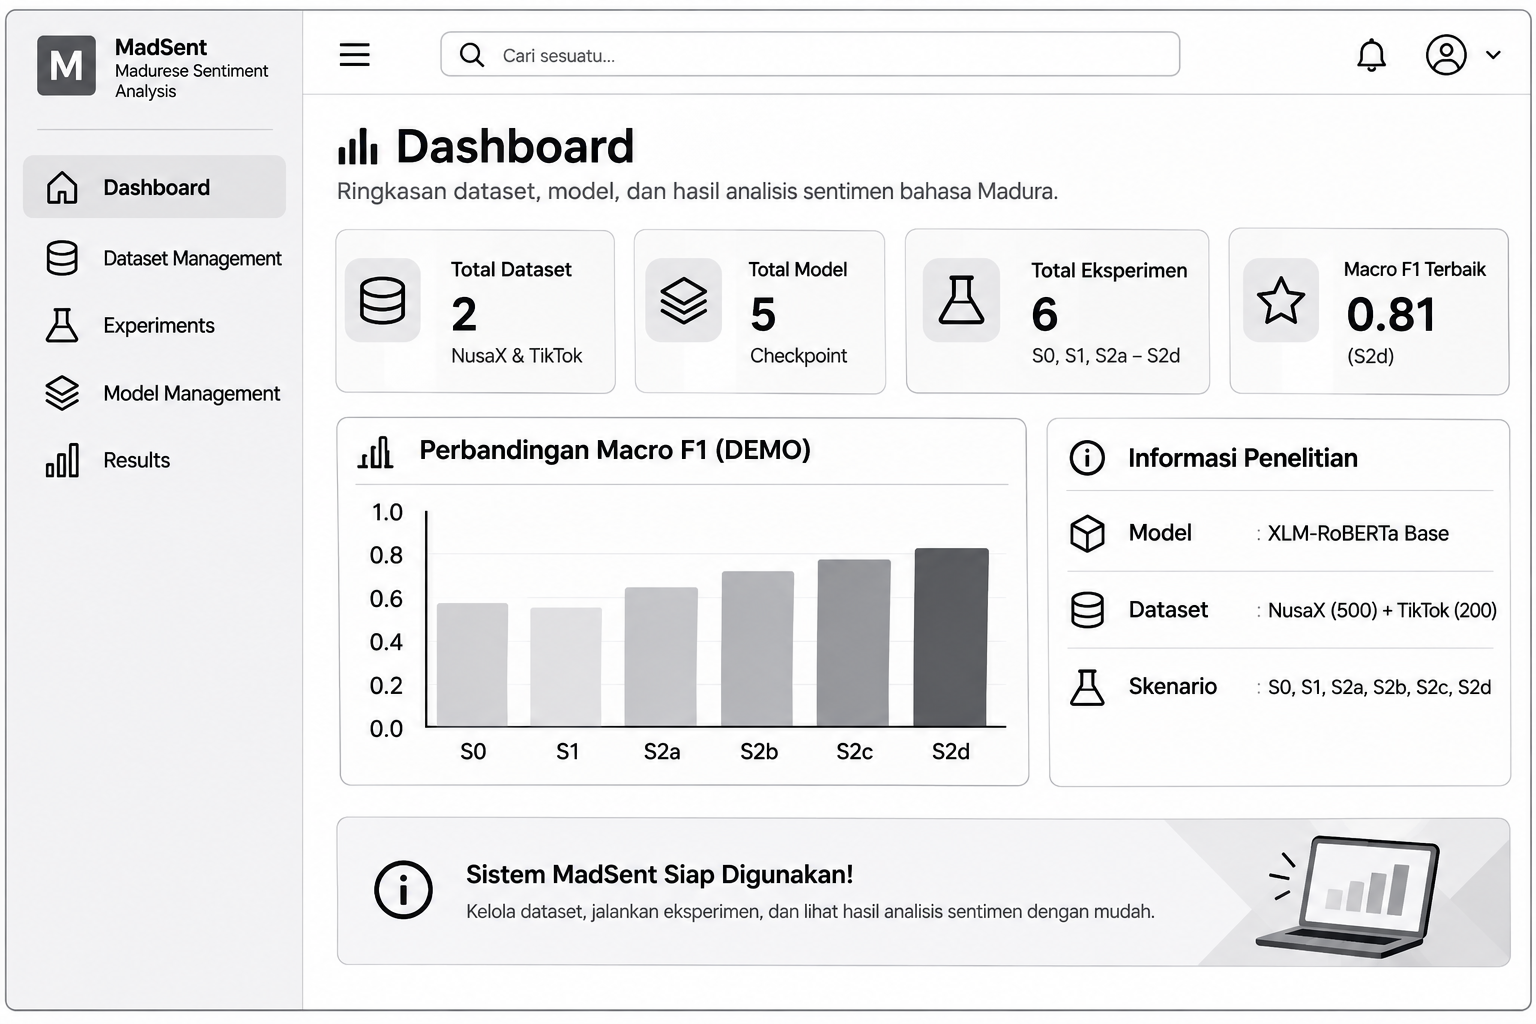
\includegraphics[width=0.68\textwidth]{figures/dashboard.png}
\caption{Rancangan Wireframe Antarmuka Modul Beranda (\textit{Dashboard})}
\label{fig:wireframe_dashboard}
\end{figure}

Sebagaimana disajikan pada \figurename~\ref{fig:wireframe_dashboard}, tata letak modul beranda memberikan gambaran komprehensif mengenai progres penelitian dan visualisasi komparatif kinerja antarskenario secara langsung, sehingga peneliti dapat memantau capaian tertinggi model secara terpadu.

\subsubsection{Modul Manajemen Data (Dataset Management)}

Modul Manajemen Data digunakan untuk mengorganisasi data teks ulasan NusaX dan komentar TikTok. Halaman ini menyediakan ringkasan volume data berlabel, fasilitas pencarian teks komentar, penyaringan berdasarkan kelas sentimen, serta tabel kurasi yang memuat ID komentar, teks bahasa Madura asli, label sentimen, dan status verifikasi. Penulis menyajikan rancangan modul manajemen data pada \figurename~\ref{fig:wireframe_dataset}.

\begin{figure}[H]
\centering
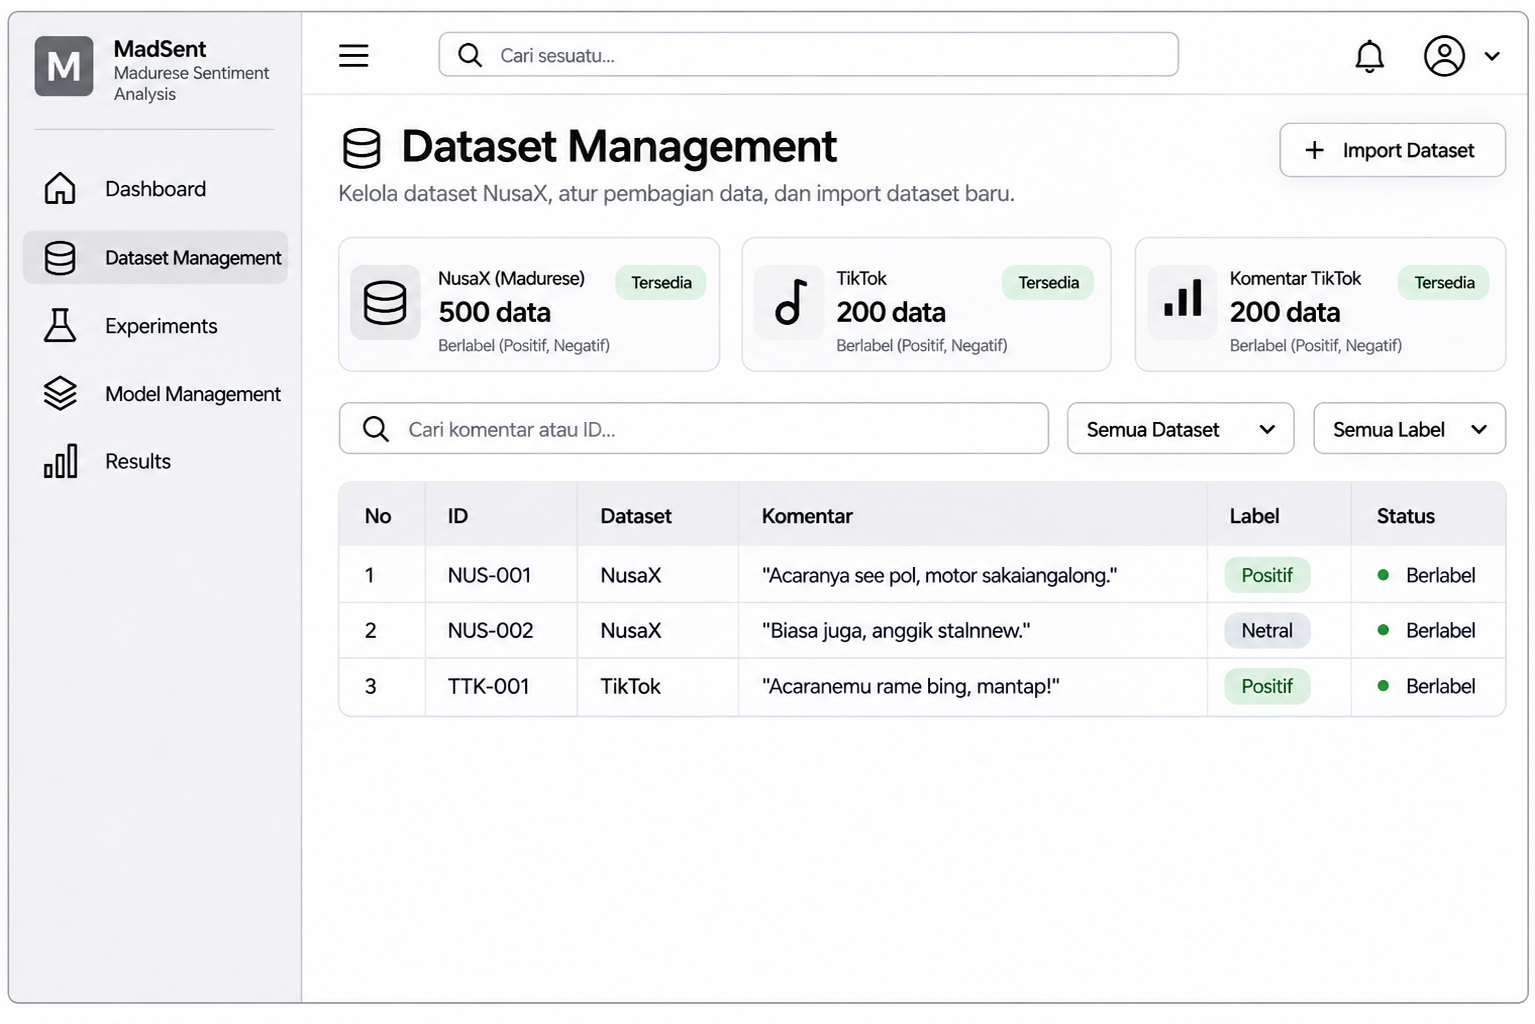
\includegraphics[width=0.68\textwidth]{figures/dataset-management.png}
\caption{Rancangan Wireframe Antarmuka Modul Manajemen Data (\textit{Dataset Management})}
\label{fig:wireframe_dataset}
\end{figure}

Sebagaimana disajikan pada \figurename~\ref{fig:wireframe_dataset}, modul manajemen data memfasilitasi penelusuran leksikon komentar daerah dan proses verifikasi label sentimen sebelum dieksekusi oleh model, serta menyediakan pemisahan tab antara korpus acuan formal dan korpus media sosial.

\subsubsection{Modul Skenario Eksperimen (Experiments)}

Modul Skenario Eksperimen mendokumentasikan keenam skenario pengujian penelitian secara runtut. Matriks eksperimen disajikan dalam format tabel interaktif yang memuat kode skenario (S0, S1, S2a, S2b, S2c, S2d), deskripsi pengujian, konfigurasi alokasi data latih, himpunan data evaluasi, dan status eksekusi. Penulis menyajikan rancangan modul skenario eksperimen pada \figurename~\ref{fig:wireframe_experiments}.

\begin{figure}[H]
\centering
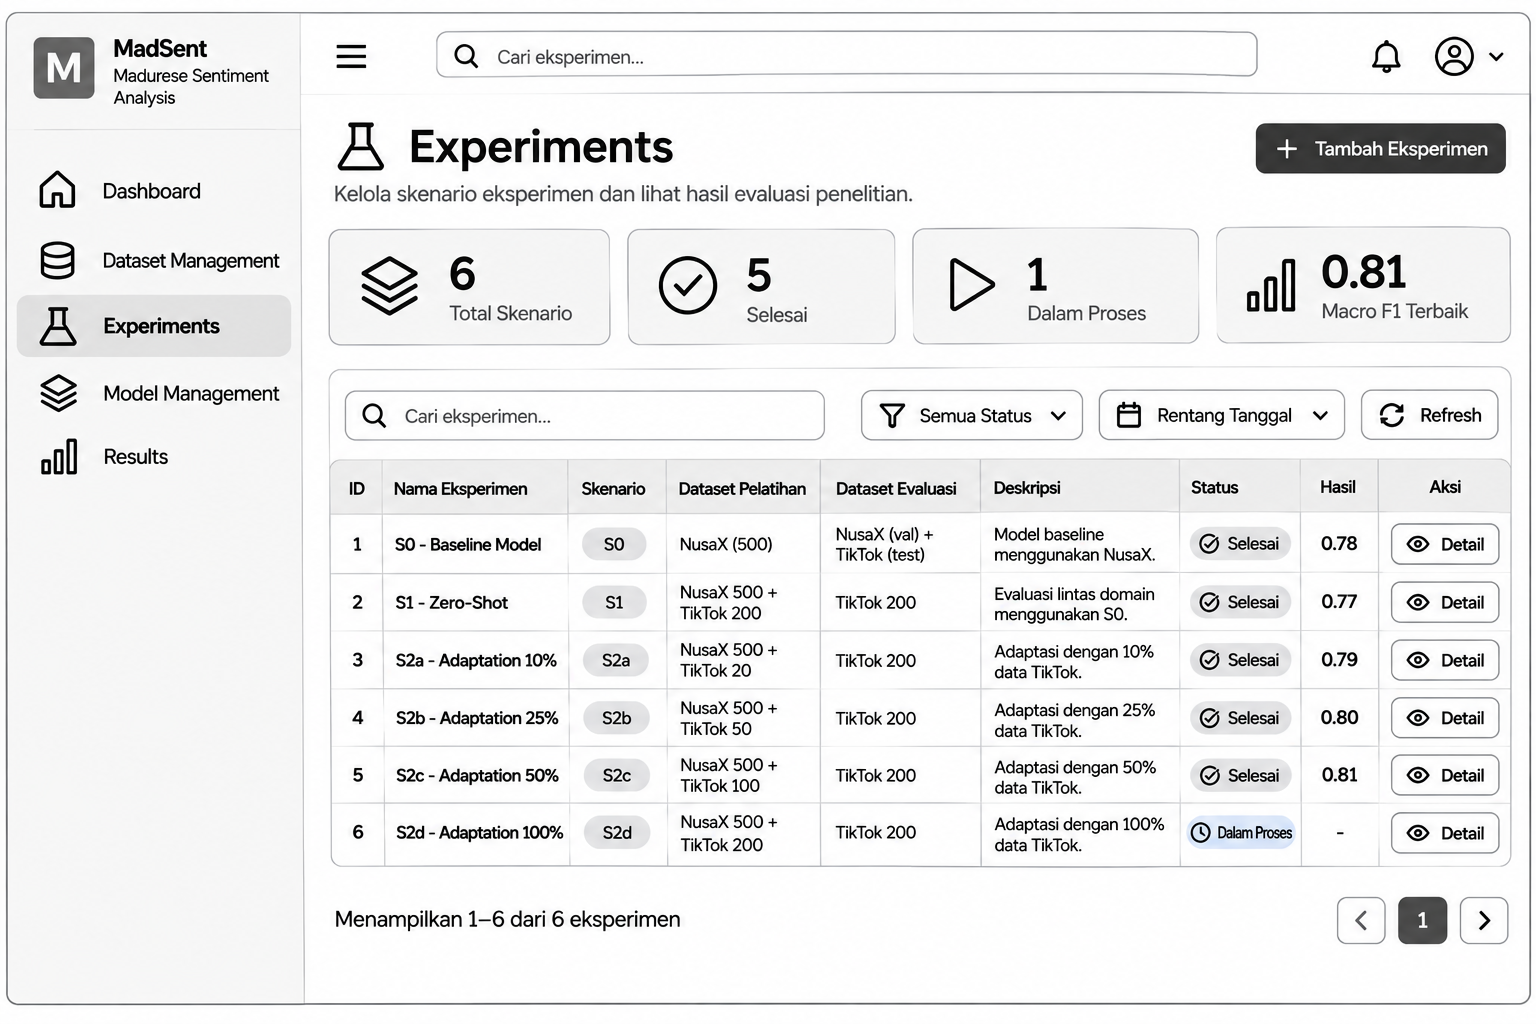
\includegraphics[width=0.68\textwidth]{figures/experiment.png}
\caption{Rancangan Wireframe Antarmuka Modul Skenario Eksperimen (\textit{Experiments})}
\label{fig:wireframe_experiments}
\end{figure}

Sebagaimana disajikan pada \figurename~\ref{fig:wireframe_experiments}, modul skenario eksperimen memastikan pencatatan konfigurasi pengujian tersimpan secara terstruktur guna mendukung replikasi hasil penelitian dan keterlacakan histori pengujian model lintas domain.

\subsubsection{Modul Manajemen Model (Model Management)}

Modul Manajemen Model berfungsi sebagai katalog pendaftaran (\textit{model registry}) untuk memantau berkas \textit{checkpoint} model XLM-RoBERTa yang telah dilatih. Pengguna dapat meninjau ketersediaan bobot model pada memori lokal, memeriksa status kesiapan pelatihan, membandingkan performa model, serta membuka laporan evaluasi model secara spesifik. Penulis menyajikan rancangan modul manajemen model pada \figurename~\ref{fig:wireframe_model}.

\begin{figure}[H]
\centering
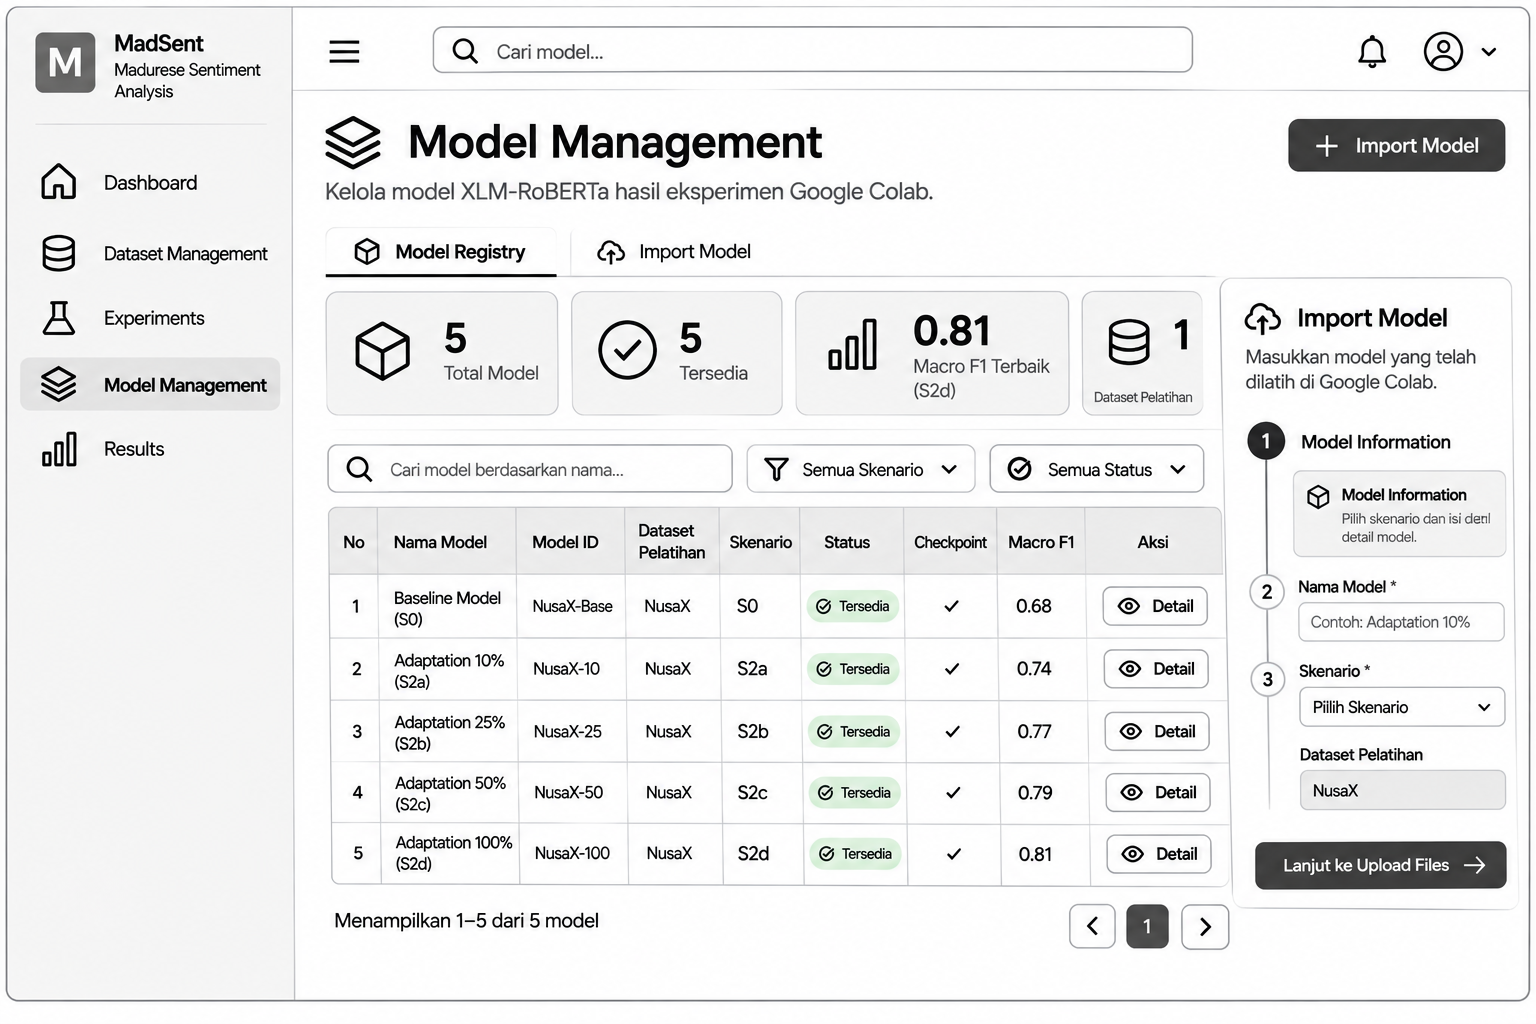
\includegraphics[width=0.68\textwidth]{figures/model-management.png}
\caption{Rancangan Wireframe Antarmuka Modul Manajemen Model (\textit{Model Management})}
\label{fig:wireframe_model}
\end{figure}

Sebagaimana disajikan pada \figurename~\ref{fig:wireframe_model}, modul manajemen model memudahkan peneliti dalam memilih dan mengaktifkan model terbaik untuk inferensi tanpa perlu melakukan pelatihan ulang, sekaligus menyediakan ringkasan metrik Macro F1 dari masing-masing checkpoint.

\subsubsection{Modul Hasil dan Evaluasi (Results)}

Modul Hasil dan Evaluasi menyajikan laporan kinerja model secara terperinci melalui kartu metrik evaluasi kuantitatif (\textit{Accuracy}, \textit{Precision}, \textit{Recall}, \textit{Macro F1-Score}), matriks konfusi interaktif tiga kelas sentimen, grafik kurva \textit{loss} pelatihan dan validasi, serta tabel analisis prediksi per komentar TikTok yang menampilkan skor keyakinan dan status kebenaran prediksi. Penulis menyajikan rancangan modul hasil dan evaluasi pada \figurename~\ref{fig:wireframe_results}.

\begin{figure}[H]
\centering
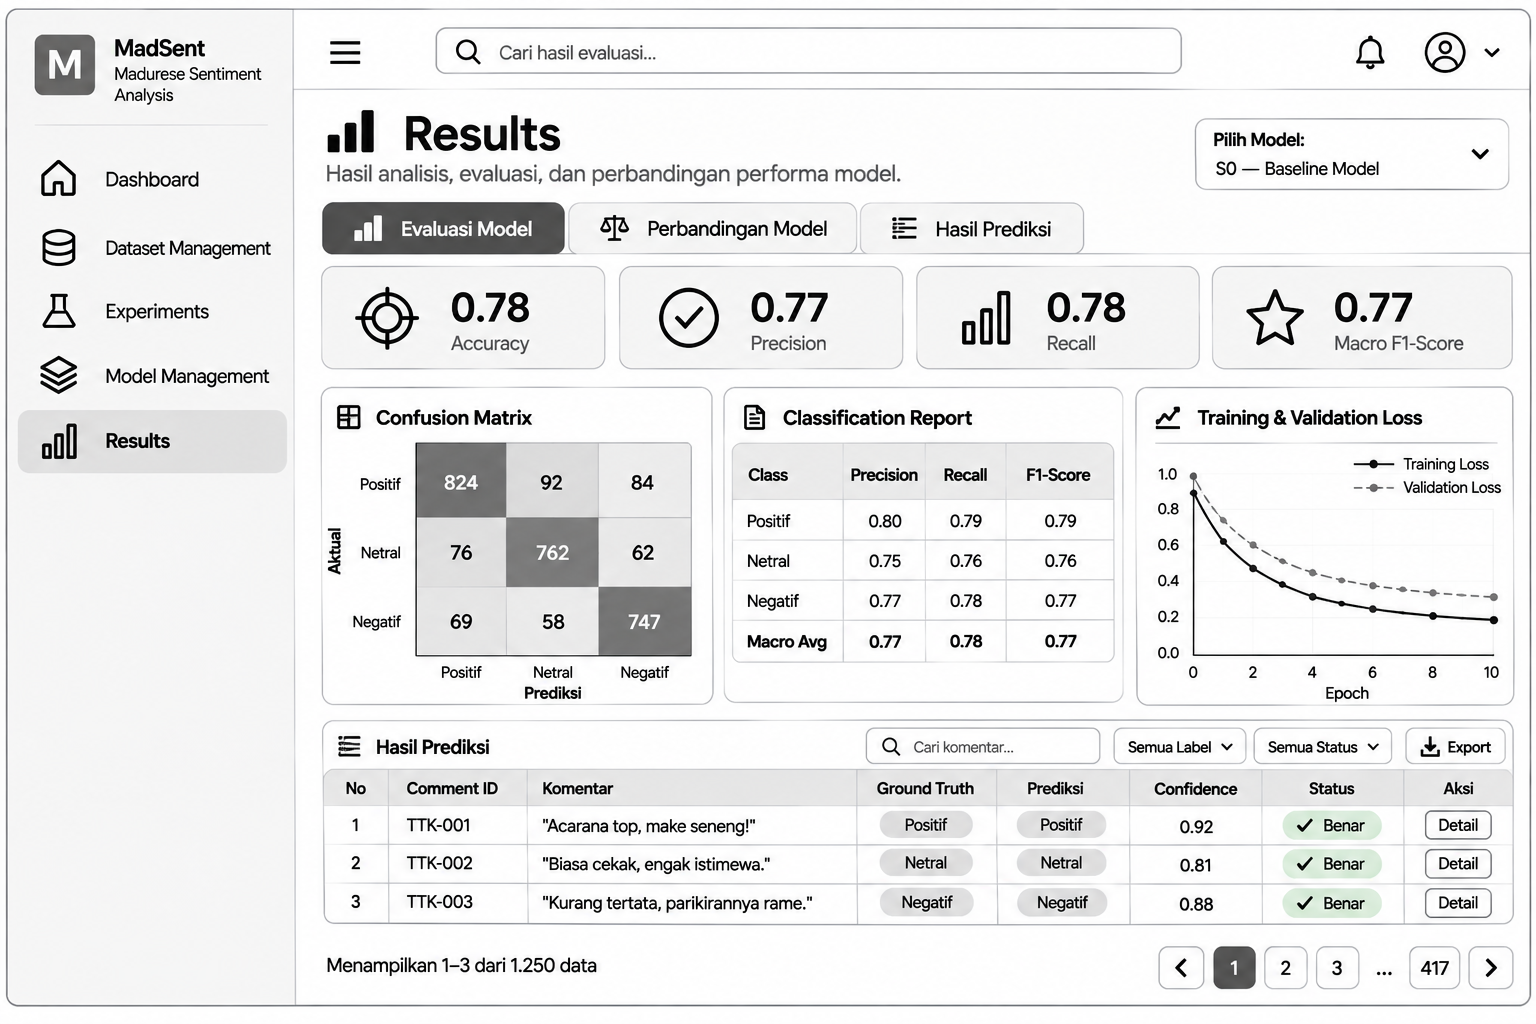
\includegraphics[width=0.68\textwidth]{figures/result.png}
\caption{Rancangan Wireframe Antarmuka Modul Hasil dan Evaluasi (\textit{Results})}
\label{fig:wireframe_results}
\end{figure}

Sebagaimana disajikan pada \figurename~\ref{fig:wireframe_results}, modul hasil dan evaluasi menyediakan sarana komprehensif bagi peneliti untuk mengidentifikasi kesalahan prediksi linguistik secara langsung pada setiap sampel komentar media sosial, sehingga memudahkan analisis mendalam pada taksonomi empat dimensi kesalahan bahasa Madura.

Melalui integrasi kelima modul antarmuka MadSent tersebut, seluruh tahapan penelitian mulai dari pengelolaan dataset, pemantauan protokol eksperimen, administrasi berkas model, hingga evaluasi kesalahan linguistik dapat dioperasikan secara terpadu dan efisien.


% ==============================================================================
% BAGIAN AKHIR (BACKMATTER)
% ==============================================================================

% Daftar Pustaka (APA Style)
\clearpage
\phantomsection
\addcontentsline{toc}{chapter}{DAFTAR PUSTAKA}
\renewcommand{\bibname}{DAFTAR PUSTAKA}
\renewcommand{\refname}{DAFTAR PUSTAKA}
\singlespacing
\bibliographystyle{apacite}
\bibliography{references/daftar-pustaka}

% Lampiran
\clearpage
% ==============================================================================
% LAMPIRAN PROPOSAL SKRIPSI
% Proposal Skripsi: Evaluasi Generalisasi Lintas Domain Model Analisis Sentimen Bahasa Madura
% Penulis: Muhammad Syawqi Muhtadabillah (NIM: 2302310276)
% ==============================================================================

\clearpage
\phantomsection
\chapter*{LAMPIRAN}
\addcontentsline{toc}{chapter}{LAMPIRAN}

\vspace{0.3cm}

% ==============================================================================
% LAMPIRAN 1: PEDOMAN OPERASIONAL ANOTASI SENTIMEN
% ==============================================================================
\section*{Lampiran 1: Pedoman Operasional Anotasi Sentimen Tiga Kelas Bahasa Madura}

Panduan ini dibuat sebagai acuan kerja bagi 2 orang penutur asli bahasa Madura yang bertindak sebagai penilai mandiri (anotator). Tugas mereka adalah menentukan label sentimen (positif, netral, atau negatif) pada 500 data komentar TikTok yang menjadi sampel penelitian.

\begin{enumerate}\singlespacing
    \item \textbf{Prinsip Dasar Anotasi}:
    \begin{itemize}
        \item Proses penilaian data dilakukan dengan melihat konteks kalimat, nada emosi, dan maksud tersirat dari penulis di media sosial. Penilaian ini sengaja menghindari penerjemahan kata demi kata secara harfiah agar makna asli dari setiap komentar tetap terjaga.
        \item Setiap komentar diberikan satu label sentimen tunggal yang saling lepas (\textit{mutually exclusive}): Positif (+1), Netral (0), atau Negatif (-1).
    \end{itemize}

    \item \textbf{Kriteria Label Positif (\textit{positive})}:
    \begin{itemize}
        \item Memuat ekspresi apresiasi, pujian, rasa senang, rasa syukur, doa keberkahan, keceriaan, atau dukungan moral terhadap kreator maupun konteks video.
        \item Sebagai contohnya: bagus (bagus), ontong (untung/bersyukur), senneng (senang), bhungah (gembira), rajen (rajin), penter (pintar), mator sakalangkong (terima kasih banyak), moga sukses, sehat teros.
    \end{itemize}

    \item \textbf{Kriteria Label Netral (\textit{neutral})}:
    \begin{itemize}
        \item Untuk kategori komentar yang netral, ciri-cirinya adalah kalimat tersebut murni hanya bertanya atau memberikan informasi tanpa ada rasa marah, senang, atau kecewa. Contohnya seperti orang yang menanyakan lokasi, menanyakan harga, meminta konfirmasi teknis, atau sekadar menyebutkan waktu dan nama orang secara datar.
        \item Contohnya adalah: dimma (di mana), arapa / a’apa (kenapa/mengapa), barempa / berempa (berapa), bila (kapan), kennengenna (tempatnya), kake / be’en (kamu), aroka (itu).
    \end{itemize}

    \item \textbf{Kriteria Label Negatif (\textit{negative})}:
    \begin{itemize}
        \item Sementara untuk kategori komentar yang negatif, ciri-cirinya sudah jelas, yaitu berisi ungkapan kemarahan, kekecewaan, atau rasa tidak suka. Kalimatnya bisa berupa ejekan, nyinyiran, keluhan tentang barang atau layanan yang jelek, hingga komentar yang tujuannya memang untuk menjatuhkan atau merendahkan orang lain.
        \item Contohnya adalah: jelek, sossa (susah/sedih), todus (malu), bheddhek (busuk), nyapcap (mengoceh tak karuan), lok penter (tidak pintar/bodoh), tadek gunana (tidak berguna), kecewa, mangkel.
    \end{itemize}

    \item \textbf{Pedoman Kasus Khusus}:
    \begin{itemize}
        \item \textbf{Sarkasme dan Satire}: Di media sosial, banyak netizen yang kalau berkomentar itu memakai sindiran atau sarkasme. Jadi, jika ada komentar yang memakai kata-kata pujian tetapi maksud aslinya adalah mengejek, komentar itu wajib kita beri nilai Negatif. Contohnya seperti kalimat: `Hebat onggu, la ancor kabbhi' yang artinya `Hebat sekali, sudah hancur semua'. Kata `hebat' di sana bukan pujian asli, melainkan cemoohan.
        \item \textbf{Campur Kode (\textit{Code-Mixing})}: Untuk komentar yang campuran bahasa Madura dan bahasa Indonesia, cara menilainya adalah dengan melihat arti keseluruhan kalimat dan apa yang paling menjadi inti bahasannya. Jadi, kita tidak menilai sepotong-sepotong per kata, melainkan melihat ke mana arah fokus komentar si netizen secara utuh.
        \item \textbf{Bahasa tidak baku}: Di TikTok, orang sering menulis kata bahasa Madura dengan ejaan yang berbeda-beda tergantung bunyinya. Contohnya, ada yang menulis dibi’ atau dhibi’, onggu atau ongghu, dan tadek atau tadhek. Menghadapi variasi ketikan ini, cara menilainya adalah dengan mengembalikan kata tersebut ke arti aslinya sesuai pemahaman orang Madura asli. Jadi, perbedaan cara mengetik ini tidak akan merusak penilaian maknanya.
    \end{itemize}
\end{enumerate}

\newpage

% ==============================================================================
% LAMPIRAN 2: FORMAT DAN INSTRUMEN LEMBAR KERJA ANOTASI
% ==============================================================================
\section*{Lampiran 2: Format dan Instrumen Lembar Kerja Anotasi Data Komentar TikTok}

Berikut adalah desain format lembar kerja (\textit{Annotation Worksheet}) yang digunakan oleh anotator penutur asli bahasa Madura untuk menginput hasil anotasi mandiri dan proses rekonsiliasi konsensus:

\begin{table}[H]
\centering
\footnotesize
\setlength{\tabcolsep}{2.5pt}
\renewcommand{\arraystretch}{1.25}
\begin{tabular}{|c|p{3.9cm}|p{2.2cm}|c|c|c|c|}
\hline
\rowcolor{gray!20}
\textbf{ID Sampel} & \textbf{Teks Komentar Asli} & \textbf{Leksikon Madura} & \textbf{A1} & \textbf{A2} & \textbf{Status} & \textbf{Konsensus} \\
\hline
TK-MAD-0001 & Mator sakalangkong tretan, videona sae onggu & sakalangkong, tretan, sae, onggu & +1 & +1 & Sesuai & Positif \\
\hline
TK-MAD-0002 & Sampeyan jualan e dimma kak? barempa hargana? & sampeyan, e dimma, barempa & 0 & 0 & Sesuai & Netral \\
\hline
TK-MAD-0003 & Pelayananna bheddhek onggu, tadek gunana pesen & bheddhek, onggu, tadek gunana & -1 & -1 & Sesuai & Negatif \\
\hline
TK-MAD-0004 & Hebat onggu barangnga, sampek ancor kabbhi & onggu, ancor, kabbhi & -1 & +1 & Diskrepansi & Negatif$^*$ \\
\hline
TK-MAD-0005 & Barangnya bagus kak, tape ongkir ka Madura larang & tape, ka Madura, larang & +1 & -1 & Diskrepansi & Positif$^{**}$ \\
\hline
TK-MAD-0006 & Mon la tak endek ya la pas mole teros & mon, tak endek, la, pas, mole & 0 & 0 & Sesuai & Netral \\
\hline
\dots & \dots & \dots & \dots & \dots & \dots & \dots \\
\hline
TK-MAD-0500 & \multicolumn{6}{l|}{\textit{[Sampel baris ke-500 korpus komentar TikTok terkurasi]}} \\
\hline
\end{tabular}
\vspace{0.1cm}
\begin{flushleft}
\footnotesize
\textit{Keterangan}: A1 = Anotator 1; A2 = Anotator 2; (+1) = Positif, (0) = Netral, (-1) = Negatif.\\
$^*$Hasil rekonsiliasi diskrepansi sarkasme: disepakati bernada negatif.\\
$^{**}$Hasil rekonsiliasi aspek ulasan produk utama: disepakati bernada positif terhadap produk.\\
\end{flushleft}
\caption{Format Instrumen Lembar Kerja Pelabelan Data Komentar TikTok}
\label{tab:format_lembar_anotasi}
\end{table}

\newpage

% ==============================================================================
% LAMPIRAN 3: FORMULASI DAN MATRIKS PENGUJIAN KESEPAKATAN ANTAR-ANOTATOR
% ==============================================================================
\section*{Lampiran 3: Formulasi dan Matriks Pengujian Kesepakatan Antar-Anotator}

Guna menjamin reliabilitas dan objektivitas pelabelan korpus data target yang melibatkan dua hingga tiga anotator penutur asli bahasa Madura, penulis melakukan pengujian kesepakatan antar-penilai untuk memastikan hasil anotasi memiliki derajat konsistensi tinggi serta bebas dari bias subjektif. Pengujian derajat reliabilitas kesepakatan antar-anotator dihitung menggunakan koefisien statistik Cohen's Kappa ($\kappa$). Rumus matematika yang digunakan adalah:
\begin{equation}
\label{eq:lampiran_kappa}
\kappa = \frac{P_o - P_e}{1 - P_e}
\end{equation}
di mana $P_o$ menyatakan proporsi kesepakatan teramati (\textit{observed agreement}), dan $P_e$ menyatakan peluang kesepakatan karena kebetulan (\textit{expected chance agreement}):
\begin{equation}
\label{eq:lampiran_pe}
P_o = \frac{\sum_{i=1}^{k} n_{ii}}{N}, \quad P_e = \sum_{i=1}^{k} \frac{n_{i\cdot} n_{\cdot i}}{N^2}
\end{equation}
dengan $N = 500$ sampel, $k = 3$ kategori sentimen, $n_{ii}$ adalah frekuensi diagnosa kesepakatan, serta $n_{i\cdot}$ dan $n_{\cdot i}$ berturut-turut adalah total marjinal baris dan kolom.

\begin{table}[H]
\centering
\footnotesize
\renewcommand{\arraystretch}{1.25}
\begin{tabular}{|l|c|c|c|c|}
\hline
\rowcolor{gray!20}
\textbf{Anotator 1 $\backslash$ Anotator 2} & \textbf{Negatif (-1)} & \textbf{Netral (0)} & \textbf{Positif (+1)} & \textbf{Total Baris} \\
\hline
\textbf{Negatif (-1)} & $n_{11}$ (Sepakat) & $n_{12}$ & $n_{13}$ & $n_{1\cdot}$ \\
\hline
\textbf{Netral (0)} & $n_{21}$ & $n_{22}$ (Sepakat) & $n_{23}$ & $n_{2\cdot}$ \\
\hline
\textbf{Positif (+1)} & $n_{31}$ & $n_{32}$ & $n_{33}$ (Sepakat) & $n_{3\cdot}$ \\
\hline
\textbf{Total Kolom} & $n_{\cdot 1}$ & $n_{\cdot 2}$ & $n_{\cdot 3}$ & $N = 500$ \\
\hline
\end{tabular}
\caption{Rancangan Matriks Kontingensi $3 \times 3$ Tabulasi Silang Antar-Anotator}
\label{tab:matriks_kontingensi}
\end{table}

\vspace{0.2cm}
Tingkat reliabilitas kesepakatan dievaluasi mengacu pada skala standar Landis \& Koch:
\begin{itemize}\singlespacing
    \item Nilai $\kappa < 0{,}20$: Kesepakatan sangat rendah (\textit{slight agreement}).
    \item Nilai $0{,}21 \le \kappa \le 0{,}40$: Kesepakatan cukup (\textit{fair agreement}).
    \item Nilai $0{,}41 \le \kappa \le 0{,}60$: Kesepakatan sedang (\textit{moderate agreement}).
    \item Nilai $0{,}61 \le \kappa \le 0{,}80$: Kesepakatan substansial (\textit{substantial agreement}).
    \item Nilai $0{,}81 \le \kappa \le 1{,}00$: Kesepakatan hampir sempurna (\textit{almost perfect agreement}).
\end{itemize}

Ambang batas penerimaan kualitas korpus dalam penelitian ini ditetapkan minimal $\kappa \ge 0{,}70$. Apabila terjadi diskrepansi label antar-anotator ($n_{ij}$ di mana $i \neq j$), dilakukan protokol rekonsiliasi bersama penutur asli senior untuk mencapai konsensus mutlak 100\% sebagai label \textit{ground truth}.

\newpage

% ==============================================================================
% LAMPIRAN 4: RENCANA JADWAL PELAKSANAAN PENELITIAN
% ==============================================================================
\section*{Lampiran 4: Rencana Jadwal Pelaksanaan Penelitian}

Pelaksanaan penelitian skripsi ini dirancang berlangsung selama 5 (lima) Minggu setelah seminar proposal dengan rincian jadwal kegiatan sebagai berikut:

\begin{table}[H]
\centering
\footnotesize
\setlength{\tabcolsep}{4pt}
\renewcommand{\arraystretch}{1.25}
\begin{tabular}{|c|>{\raggedright\arraybackslash}p{5.2cm}|c|c|c|c|c|}
\hline
\rowcolor{gray!20}
\textbf{No} & \textbf{Tahapan Kegiatan Penelitian} & \textbf{Mgg 1} & \textbf{Mgg 2} & \textbf{Mgg 3} & \textbf{Mgg 4} & \textbf{Mgg 5} \\
\hline
1 & Seminar Proposal \& Penyempurnaan Usulan & $\blacksquare$ & & & & \\
\hline
2 & Pengambilan Data Manual Komentar TikTok & $\blacksquare$ & $\blacksquare$ & & & \\
\hline
3 & Kurasi Leksikon Madura \& Pra-pemrosesan Teks & & $\blacksquare$ & & & \\
\hline
4 & Pelabelan Korpus oleh 2 Penutur Asli & & $\blacksquare$ & & & \\
\hline
5 & Uji Reliabilitas Kappa \& Rekonsiliasi Konsensus & & $\blacksquare$ & & & \\
\hline
6 & Partisi Korpus Terstratifikasi (Test, Val, Pool) & & & $\blacksquare$ & & \\
\hline
7 & Pelatihan Baseline XLM-RoBERTa di NusaX & & & $\blacksquare$ & & \\
\hline
8 & Pengujian Zero-Shot Cross-Domain ke TikTok & & & $\blacksquare$ & $\blacksquare$ & \\
\hline
9 & Eksperimen Adaptasi Bertahap (10\%, 25\%, 50\%, 100\%) & & & & $\blacksquare$ & \\
\hline
10 & Evaluasi Metrik Macro F1 \& Analisis Error Linguistik & & & & $\blacksquare$ & \\
\hline
11 & Penyusunan Laporan Lengkap Skripsi (Bab IV--V) & & & & $\blacksquare$ & $\blacksquare$ \\
\hline
12 & Ujian Sidang Akhir Skripsi & & & & & $\blacksquare$ \\
\hline
\end{tabular}
\vspace{0.1cm}
\begin{flushleft}
\footnotesize
\textit{Keterangan}: Tanda ($\blacksquare$) menunjukkan alokasi waktu pelaksanaan kegiatan per bulan.\\
\end{flushleft}
\caption{Rencana Jadwal Pelaksanaan Penelitian (Gantt Chart)}
\label{tab:jadwal_penelitian}
\end{table}


\end{document}
